\documentclass[manuscript,nonacm,anonymous]{acmart}
\usepackage{algorithm}
\usepackage{algpseudocode} % for pseudocode
\usepackage{tikz} % for figures
\usepackage{subcaption} % for subfigures
\usetikzlibrary{decorations.pathreplacing}

\hyphenation{time-stamp time-stamps re-con-cilia-tion data-center}
\renewcommand{\floatpagefraction}{.8}%

% Custom macros
\newcommand{\I}{$\mathcal{I}\!$}

\begin{document}
\title{Causal Broadcast with Arbitrarily Many Byzantine Nodes}

\author{Martin Kleppmann}
\orcid{0000-0001-7252-6958}
\affiliation{%
  \institution{University of Cambridge}
  \city{Cambridge}
  \country{UK}
}
\email{mk428@cst.cam.ac.uk}


\author{Heidi Howard}
\orcid{0000-0001-5256-7664}
\affiliation{%
  \institution{University of Cambridge}
  \city{Cambridge}
  \country{UK}
}
\email{hh360@cst.cam.ac.uk}

%\begin{CCSXML}
%<ccs2012>
%  <concept>
%    <concept_id>10003752.10003809.10010172</concept_id>
%    <concept_desc>Theory of computation~Distributed algorithms</concept_desc>
%    <concept_significance>500</concept_significance>
%  </concept>
%  <concept>
%    <concept_id>10002951.10003152.10003166.10003172</concept_id>
%    <concept_desc>Information systems~Remote replication</concept_desc>
%    <concept_significance>300</concept_significance>
%  </concept>
%  <concept>
%    <concept_id>10010520.10010575</concept_id>
%    <concept_desc>Computer systems organization~Dependable and fault-tolerant systems and networks</concept_desc>
%    <concept_significance>300</concept_significance>
%  </concept>
%  <concept>
%    <concept_id>10002978.10003014.10003015</concept_id>
%    <concept_desc>Security and privacy~Security protocols</concept_desc>
%    <concept_significance>300</concept_significance>
%  </concept>
%</ccs2012>
%\end{CCSXML}

%\ccsdesc[500]{Theory of computation~Distributed algorithms}
%\ccsdesc[300]{Information systems~Remote replication}
%\ccsdesc[300]{Computer systems organization~Dependable and fault-tolerant systems and networks}
%\ccsdesc[300]{Security and privacy~Security protocols}

%\keywords{replication, Byzantine fault tolerance, eventual consistency, CRDTs, broadcast protocols}

\begin{abstract}
Sybil attacks, in which a large number of adversary-controlled nodes join a network, are a concern for many permissionless decentralized systems, necessitating expensive countermeasures such as proof-of-work.
However, there is a category of distributed applications that are, by design, immune to Sybil attacks because they can tolerate arbitrary numbers of Byzantine-faulty nodes.
In this paper, we show that causal broadcast falls within this category by demonstrating a Byzantine fault tolerant algorithm for causal broadcast, proving it correct, and demonstrating near-optimal performance in a prototype implementation.
Our algorithm can be used to implement replicated storage systems, such as some types of distributed ledger, which need to withstand Byzantine faults.
\end{abstract}
\maketitle

% TODO: Frame our protocol as a type of distributed ledger?

\section{Introduction}

Peer-to-peer systems are of interest to many communities for a number of reasons: their lack of central control by a single party can make them more resilient, and less susceptible to censorship and denial-of-service attacks than centralized services.
Examples of widely deployed peer-to-peer applications include file sharing~\cite{Pouwelse:2005,Benet:2014}, scientific dataset sharing~\cite{Robinson:2018}, decentralized social networking~\cite{Tarr:2019}, cryptocurrencies~\cite{Nakamoto:2008}, and blockchains~\cite{Bano:2019}.

The central challenge faced by these decentralized systems is that peers cannot be trusted because anybody in the world can add peers to the network.
Thus, we must assume that some subset of peers are malicious; such peers are also called \emph{Byzantine-faulty}, which means that they may deviate from the specified protocol in arbitrary ways.
Moreover, a malicious party may perform a \emph{Sybil attack}~\cite{Douceur:2002}: launching a large number of peers, potentially causing the Byzantine-faulty peers to outnumber the honest ones.

Several countermeasures against Sybil attacks are used.
Bitcoin popularized the concept of \emph{proof-of-work}~\cite{Nakamoto:2008}, in which a peer's voting power depends on the computational effort it expends.
Unfortunately, proof-of-work is extraordinarily expensive: it has been estimated that as of 2020, Bitcoin alone represents almost half of worldwide datacenter electricity use~\cite{deVries:2020}.
Other mechanisms, such as \emph{proof-of-stake}~\cite{Bano:2019}, are at present unproven at scale.
\emph{Permissioned} blockchains avoid this huge carbon footprint, but they have the downside of requiring central control over the peers that may join the system, undermining the principle of decentralization.

The reason why permissioned blockchains must control membership is that they rely on Byzantine agreement, which assumes that at most $f$ nodes are Byzantine-faulty.
To tolerate $f$ faults, Byzantine agreement algorithms typically require at least $3f+1$ nodes~\cite{Castro:1999}.
% It is well established that without synchrony, Byzantine agreement is impossible if $n<3f+1$~\cite{Dwork:1988,Lamport:1982}.
If more than $f$ nodes are faulty, these algorithms can guarantee neither safety (agreement) nor liveness (progress).
Thus, a Sybil attack that causes the bound of $f$ faulty nodes to be exceeded can result in the system's guarantees being violated; for example, in a cryptocurrency, they could allow the same coin to be spent multiple times (a \emph{double-spending} attack).

This state of affairs raises the question: if Byzantine agreement cannot be achieved in the face of arbitrary numbers of Byzantine-faulty nodes, what properties \emph{can} be guaranteed in this case?
A system that tolerates arbitrary numbers of Byzantine-faulty nodes is immune to Sybil attacks: even if the malicious peers outnumber the honest ones, it is still able to function correctly.
Such a system requires neither proof-of-work nor the central control of permissioned blockchains, opening up new possibilities for the design of trustless decentralized systems.

Our contributions in this paper are as follows:
\begin{enumerate}
    \item We show that causal broadcast can be achieved in systems with arbitrary numbers of Byzantine-faulty nodes by defining an algorithm for \emph{Byzantine causal broadcast} (Section~\ref{sec:algorithm}), a mechanism for reliably disseminating messages to a group of nodes, and proving its correctness (Appendix~\ref{sec:proof}).
    \item We experimentally evaluate the performance of our algorithm, and demonstrate that it incurs significantly lower communication costs (in terms of round trips and message size) than existing algorithms (Section~\ref{sec:evaluation}).
    \item We highlight how Byzantine causal broadcast can be used to implement replicated storage systems and distributed applications that are immune to Sybil attacks (Section~\ref{sec:applications}).
\end{enumerate}


\section{Background}

\subsection{System model}\label{sec:system-model}

Our system consists of a finite set of nodes, which may vary over time.
Each node is either \emph{correct} or \emph{faulty}, but a correct node does not know whether another node is faulty.
A correct node is not crashed and follows the specified protocol, whereas a faulty node may deviate from the protocol in arbitrary ways (i.e.\ it is Byzantine-faulty~\cite{Lamport:1982}).
Faulty nodes may collude and attempt to deceive correct nodes; we model such worst-case behavior by assuming a malicious adversary who controls the behavior of all faulty nodes.
We allow any subset of nodes to be faulty.
We consider all nodes to be equal peers, making no distinction e.g.\ between clients and servers.
Nodes may crash and recover; as long as a crashed node eventually recovers, and otherwise follows the protocol, we still call it ``correct''.

We assume that each node has a distinct private key that can be used for digital signatures, and that the corresponding public key is known to all nodes.
We assume that no node knows the private key of another node, and thus signatures cannot be forged.
Unlike in a permissioned blockchain, there is no need for central control over the set of public keys in the system: for example, one node may add another node to the system by informing the existing nodes about the new node's public key.

Nodes communicate by sending messages over pairwise (bidirectional, unicast) network links.
We assume that all messages sent over these links are authenticated with the sender's private key, and the recipient ignores messages with invalid signatures.
Thus, even if the adversary can tamper with network traffic, it can only cause message loss but not impersonate a correct node.
For simplicity, our algorithms assume that network links are reliable, i.e.\ that a sent message is eventually delivered, provided that neither sender nor recipient crashes.
This can easily be achieved by detecting and retransmitting any lost messages.

We make no timing assumptions: messages may experience unbounded delay in the network (for example, due to retransmissions during temporary network partitions), nodes may execute at different speeds, and we do not assume any clock synchronization (i.e.\ we assume an \emph{asynchronous} system model).
We do assume that a node has a timer that allows it to perform some task approximately periodically, such as retransmitting unacknowledged messages, without requiring exact time measurement.

\begin{figure}
    \centering
    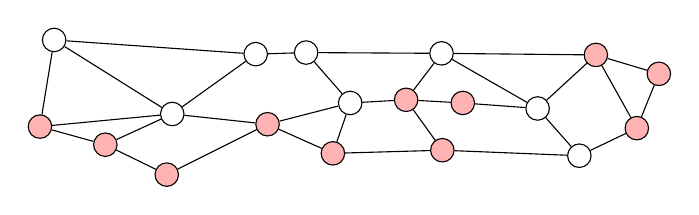
\begin{tikzpicture}
\tikzstyle{correct}=[draw,circle,inner sep=3pt]
\tikzstyle{faulty}=[draw,circle,inner sep=3pt,fill=red!30]
\node [faulty] (a) at (0.04,0.70) {};
\node [correct] (b) at (0.22,1.80) {};
\node [faulty] (c) at (0.87,0.47) {};
\node [correct] (d) at (1.72,0.86) {};
\node [faulty] (e) at (1.65,0.09) {};
\node [correct] (f) at (2.78,1.62) {};
\node [faulty] (g) at (2.93,0.73) {};
\node [correct] (h) at (3.42,1.64) {};
\node [faulty] (i) at (3.76,0.36) {};
\node [correct] (j) at (3.98,1.00) {};
\node [faulty] (k) at (4.69,1.04) {};
\node [correct] (l) at (5.14,1.63) {};
\node [faulty] (m) at (5.15,0.40) {};
\node [faulty] (n) at (5.41,1.00) {};
\node [correct] (o) at (6.36,0.93) {};
\node [correct] (p) at (6.89,0.33) {};
\node [faulty] (q) at (7.10,1.61) {};
\node [faulty] (r) at (7.62,0.68) {};
\node [faulty] (s) at (7.90,1.37) {};
\draw (a) -- (b);
\draw (a) -- (c);
\draw (a) -- (d);
\draw (b) -- (d);
\draw (b) -- (f);
\draw (c) -- (d);
\draw (c) -- (e);
\draw (d) -- (f);
\draw (d) -- (g);
\draw (e) -- (g);
\draw (f) -- (h);
\draw (g) -- (i);
\draw (g) -- (j);
\draw (h) -- (j);
\draw (h) -- (l);
\draw (i) -- (j);
\draw (i) -- (m);
\draw (j) -- (k);
\draw (k) -- (l);
\draw (k) -- (m);
\draw (k) -- (n);
\draw (l) -- (o);
\draw (l) -- (q);
\draw (m) -- (p);
\draw (n) -- (o);
\draw (o) -- (p);
\draw (o) -- (q);
\draw (p) -- (r);
\draw (q) -- (s);
\draw (q) -- (r);
\draw (r) -- (s);
\end{tikzpicture}

\vspace{0.5cm}
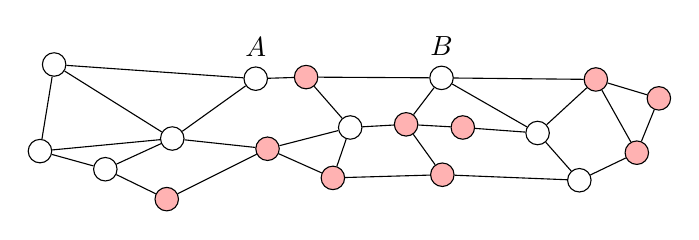
\begin{tikzpicture}
\tikzstyle{correct}=[draw,circle,inner sep=3pt]
\tikzstyle{faulty}=[draw,circle,inner sep=3pt,fill=red!30]
\node [correct] (a) at (0.04,0.70) {};
\node [correct] (b) at (0.22,1.80) {};
\node [correct] (c) at (0.87,0.47) {};
\node [correct] (d) at (1.72,0.86) {};
\node [faulty] (e) at (1.65,0.09) {};
\node [correct] (f) at (2.78,1.62) {};
\node [faulty] (g) at (2.93,0.73) {};
\node [faulty] (h) at (3.42,1.64) {};
\node [faulty] (i) at (3.76,0.36) {};
\node [correct] (j) at (3.98,1.00) {};
\node [faulty] (k) at (4.69,1.04) {};
\node [correct] (l) at (5.14,1.63) {};
\node [faulty] (m) at (5.15,0.40) {};
\node [faulty] (n) at (5.41,1.00) {};
\node [correct] (o) at (6.36,0.93) {};
\node [correct] (p) at (6.89,0.33) {};
\node [faulty] (q) at (7.10,1.61) {};
\node [faulty] (r) at (7.62,0.68) {};
\node [faulty] (s) at (7.90,1.37) {};
\draw (a) -- (b);
\draw (a) -- (c);
\draw (a) -- (d);
\draw (b) -- (d);
\draw (b) -- (f);
\draw (c) -- (d);
\draw (c) -- (e);
\draw (d) -- (f);
\draw (d) -- (g);
\draw (e) -- (g);
\draw (f) -- (h);
\draw (g) -- (i);
\draw (g) -- (j);
\draw (h) -- (j);
\draw (h) -- (l);
\draw (i) -- (j);
\draw (i) -- (m);
\draw (j) -- (k);
\draw (k) -- (l);
\draw (k) -- (m);
\draw (k) -- (n);
\draw (l) -- (o);
\draw (l) -- (q);
\draw (m) -- (p);
\draw (n) -- (o);
\draw (o) -- (p);
\draw (o) -- (q);
\draw (p) -- (r);
\draw (q) -- (s);
\draw (q) -- (r);
\draw (r) -- (s);
\path (f.north) node [above] {$A$};
\path (l.north) node [above] {$B$};
\end{tikzpicture}

    \caption{Above: correct nodes (white) form a connected component. Below: faulty nodes (red) are able to prevent communication between correct nodes $p$ and $q$.}
    \label{fig:connected}
\end{figure}

Not all pairs of nodes are necessarily connected with a network link.
However, we must assume that in the graph of nodes and network links, the correct nodes form a single connected component, as illustrated in Figure~\ref{fig:connected}.
This assumption is necessary because if two correct nodes can only communicate via faulty nodes, then no algorithm can guarantee data exchange between those nodes, as the adversary can always block communication (this is known as an \emph{eclipse attack}~\cite{Singh:2004}).
The easiest way of satisfying this assumption is to connect each node to every other.

\subsection{Reliable, causal, and total order broadcast}\label{sec:broadcast}

A broadcast protocol is an abstraction that allows one node to send a message to all nodes in the system.
Broadcast protocols are defined in terms of two primitives, \emph{broadcast} and \emph{deliver}.
We consider three variants: reliable broadcast, total order broadcast, and causal broadcast.

\emph{Reliable broadcast} algorithms must satisfy the following properties~\cite{Cachin:2011wt}:

\begin{description}
\item[Self-delivery:] If a correct node $p$ broadcasts a message $m$, then $p$ eventually delivers $m$.
\item[Eventual delivery:] If a correct node delivers a message $m$, then all correct nodes will eventually deliver $m$.
\item[Authenticity:] If a correct node delivers a message $m$ with sender $s$, then $m$ was previously broadcast by $s$.
\item[Non-duplication:] A correct node does not deliver the same message more than once.
\end{description}

Reliable broadcast does not constrain the order in which messages may be delivered.
In many applications the delivery order is important, so we can strengthen the model.
For example, \emph{total order broadcast} must satisfy the four properties of reliable broadcast, and additionally the following property:

\begin{description}
\item[Total order:] If a correct node delivers message $m_1$ before delivering message $m_2$, then all correct nodes must deliver $m_1$ before delivering $m_2$.
\end{description}

Total order broadcast ensures that all nodes deliver the same messages in the same order~\cite{Defago:2004ji}.
It is a very powerful model, since it can implement \emph{state machine replication}~\cite{Schneider:1990} (providing linearizable replicated storage).

In a Byzantine system, total order broadcast is implemented by Byzantine agreement algorithms.
An example is a blockchain, in which the totally ordered chain of blocks corresponds to the sequence of delivered messages~\cite{Bano:2019}.
However, Byzantine agreement algorithms must assume a maximum number of faulty nodes (see Section~\ref{sec:relwork}), and hence require Sybil countermeasures.
To ensure eventual delivery they must also assume partial synchrony~\cite{Dwork:1988}.

%State machine replication treats every node as a deterministic state machine, where the inputs are commands.
%If all nodes observe the same commands in the same order, they all go through the same sequence of state transitions, resulting in the same final state.

\emph{Causal broadcast}~\cite{Birman:1991el,Cachin:2011wt} must satisfy the four properties of reliable broadcast, and additionally the following ordering property, which is weaker than total order:

\begin{description}
\item[Causal order:] If a correct node broadcasts or delivers $m_1$ before broadcasting message $m_2$, then all correct nodes must deliver $m_1$ before delivering $m_2$.
\end{description}

Causal order is based on the observation that when a node broadcasts a message, that message may depend on prior messages seen by that node (these are \emph{causal dependencies}).
It then imposes a partial order on messages: $m_1$ must be delivered before $m_2$ if $m_2$ has a causal dependency on $m_1$.
Concurrently sent messages, which do not depend on each other, can be delivered in any order.

\begin{figure}
\begin{subfigure}{0.49\columnwidth}
    \centering
    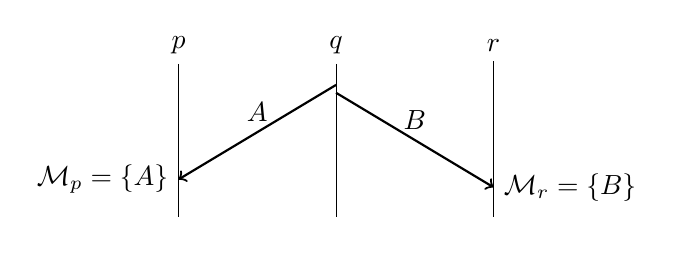
\begin{tikzpicture}
% Timelimes
\node (p-start) at (0, 0.5) {$p$};
\node (p-end)   at (0, -1.8) {};
\node (q-start) at (2, 0.5) {$q$};
\node (q-end)   at (2, -1.8) {};
\node (r-start) at (4, 0.5) {$r$};
\node (r-end)   at (4, -1.8) {};
\draw (p-start) -- (p-end);
\draw (q-start) -- (q-end);
\draw (r-start) -- (r-end);

% Messages
\draw[thick,->] (2, 0) to node [above] {$A$} (0, -1.2) node [left] {$\mathcal{M}_p = \{A\}$};

\draw[thick,->] (2, -0.1) to node [above] {$B$} (4, -1.3) node [right] {$\mathcal{M}_r = \{B\}$};

\end{tikzpicture}

    \captionsetup{width=.95\linewidth}
    \caption{Byzantine-faulty node $q$ sends conflicting messages to correct nodes $p$ and $r$.
    The sets $\mathcal{M}_p$ and ${M}_r$ do not converge.}
    \label{fig:trivial1}
\end{subfigure}
\begin{subfigure}{0.49\columnwidth}
    \centering
    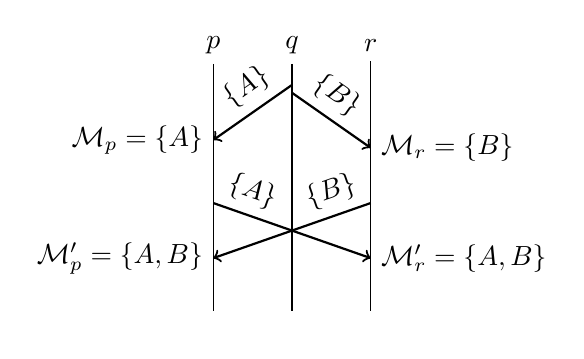
\begin{tikzpicture}

% Space between timelines
\def\width{1}
% Message delay
\def\delay{0.7}

% Timelimes
\node (p-start) at (0, 0.5) {$p$};
\node (p-end)   at (0, -3) {};
\node (q-start) at (\width, 0.5) {$q$};
\node (q-end)   at (\width, -3) {};
\node (r-start) at (\width*2, 0.5) {$r$};
\node (r-end)   at (\width*2, -3) {};
\draw (p-start) -- (p-end);
\draw (q-start) -- (q-end);
\draw (r-start) -- (r-end);

% Messages
\draw[thick,->] (\width, 0) to node [above,pos=0.4,sloped] {$\{A\}$} (0, -\delay) node [left] {$\mathcal{M}_p = \{A\}$};

\draw[thick,->] (\width, -0.1) to node [above,pos=0.4,sloped] {$\{B\}$} (\width*2, -\delay-0.1) node [right] {$\mathcal{M}_r = \{B\}$};

\draw[thick,->] (0, -1.5) to node [above,pos=0.2,sloped] {$\{A\}$} (\width*2, -1.5-\delay) node [right] {$\mathcal{M}_r' = \{A,B\}$};

\draw[thick,->] (\width*2, -1.5) to node [above,pos=0.2,sloped] {$\{B\}$} (0, -1.5-\delay) node [left] {$\mathcal{M}_p' = \{A,B\}$};

\end{tikzpicture}

% \begin{tikzpicture}
% % Timelimes
% \node (p-start) at (0, 0.5) {$p$};
% \node (p-end)   at (0, -3.4) {};
% \node (q-start) at (2, 0.5) {$q$};
% \node (q-end)   at (2, -3.4) {};
% \node (r-start) at (4, 0.5) {$r$};
% \node (r-end)   at (4, -3.4) {};
% \draw (p-start) -- (p-end);
% \draw (q-start) -- (q-end);
% \draw (r-start) -- (r-end);

% % Messages
% \draw[thick,->] (2, 0) to node [above] {$\{A\}$} (0, -1.2) node [left] {$\mathcal{M}_p = \{A\}$};

% \draw[thick,->] (2, -0.1) to node [above] {$\{B\}$} (4, -1.3) node [right] {$\mathcal{M}_r = \{B\}$};

% \draw[thick,->] (0, -1.7) to node [above,pos=0.25] {$\{A\}$} (4, -2.9) node [right] {$\mathcal{M}_r' = \{A,B\}$};

% \draw[thick,->] (4, -1.7) to node [above,pos=0.25] {$\{B\}$} (0, -2.9) node [left] {$\mathcal{M}_p' = \{A,B\}$};

% \end{tikzpicture}

    \captionsetup{width=.95\linewidth}
    \caption{As correct nodes $p$ and $r$ reconcile their sets of messages, they converge to the same set $\mathcal{M}_p' = \mathcal{M}_r' = \{A,B\}$.}
    \label{fig:trivial2}
\end{subfigure}
\caption{Ensuring that all correct eventually deliver the same set of messages.}
\end{figure}

\subsection{Na\"{\i}ve broadcast algorithms}\label{sec:naive-broadcast-algorithms}

The simplest broadcast algorithm is as follows: every time a node wants to broadcast a message, it delivers that message to itself, and also sends that message to each other node via a pairwise network link, re-transmitting until it is acknowledged.
However, this algorithm does not provide the \emph{eventual delivery} property in the face of Byzantine-faulty nodes, as shown in Figure~\ref{fig:trivial1}: a faulty node $q$ may send two different messages $A$ and $B$ to correct nodes $p$ and $r$, respectively; then $p$ never delivers $B$ and $r$ never delivers $A$.

To address this issue, nodes $p$ and $r$ must communicate with each other (either directly, or indirectly via other correct nodes).
Let $\mathcal{M}_p$ and $\mathcal{M}_r$ be the set of messages delivered by nodes $p$ and $r$, respectively.
As shown in Figure~\ref{fig:trivial2}, $p$ can send its entire set $\mathcal{M}_p$ to $r$, and $r$ can send $\mathcal{M}_r$ to $p$, so that both nodes can compute $\mathcal{M}_p \cup \mathcal{M}_r$, and deliver any new messages.
Pairs of nodes can thus periodically \emph{reconcile} their sets of delivered messages.

Adding this reconciliation process to the protocol ensures reliable broadcast.
However, this algorithm is very inefficient: when nodes periodically reconcile their state, we can expect that at the start of each round of reconciliation their sets of messages already have many elements in common.
Sending the entire set of messages to each other transmits a large amount of data unnecessarily.

An efficient reconciliation algorithm should determine which messages have already been delivered by both nodes, and transmit only those messages that are unknown to the other node.
For example, node $p$ should only send $\mathcal{M}_p \setminus \mathcal{M}_r$ to node $r$, and node $r$ should only send $\mathcal{M}_r \setminus \mathcal{M}_p$ to node $p$.
The algorithm should also complete in a small number of round-trips and minimize the size of messages sent.
These goals rule out other na\"{\i}ve approaches too: for example, instead of sending all messages in $\mathcal{M}_p$, node $p$ could send the hash of each message in $\mathcal{M}_p$, which can be used by other nodes to determine which messages they are missing; this is still inefficient, as the message size is $O(|\mathcal{M}_{p}|)$.

\begin{figure*}
    \centering
    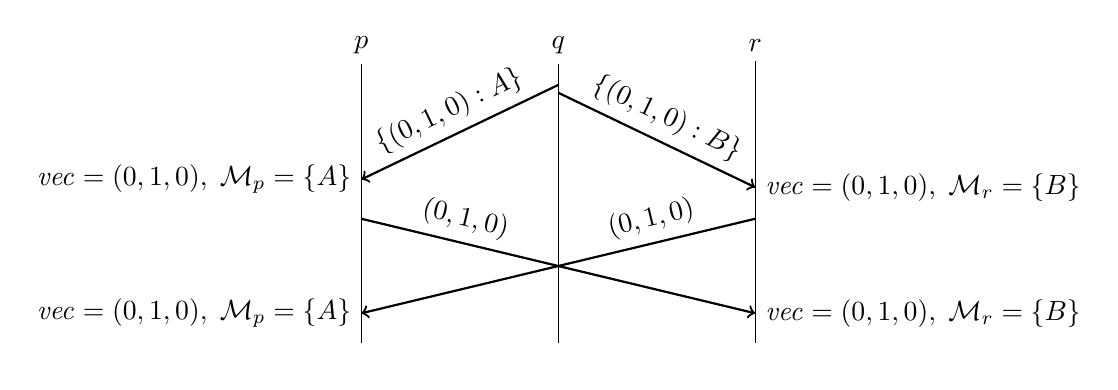
\begin{tikzpicture}
% Timelimes
\node (p-start) at (0, 0.5) {$p$};
\node (p-end)   at (0, -3.4) {};
\node (q-start) at (2.5, 0.5) {$q$};
\node (q-end)   at (2.5, -3.4) {};
\node (r-start) at (5, 0.5) {$r$};
\node (r-end)   at (5, -3.4) {};
\draw (p-start) -- (p-end);
\draw (q-start) -- (q-end);
\draw (r-start) -- (r-end);

% Messages
\draw[thick,->] (2.5, 0) to node [above,sloped] {$\{(0,1,0): A\}$} (0, -1.2) node [left] {$\mathit{vec} = (0,1,0),\; \mathcal{M}_p = \{A\}$};

\draw[thick,->] (2.5, -0.1) to node [above,sloped] {$\{(0,1,0): B\}$} (5, -1.3) node [right] {$\mathit{vec} = (0,1,0),\; \mathcal{M}_r = \{B\}$};

\draw[thick,->] (0, -1.7) to node [above,pos=0.25,sloped] {$(0,1,0)$} (5, -2.9) node [right] {$\mathit{vec} = (0,1,0),\; \mathcal{M}_r = \{B\}$};

\draw[thick,->] (5, -1.7) to node [above,pos=0.25,sloped] {$(0,1,0)$} (0, -2.9) node [left] {$\mathit{vec} = (0,1,0),\; \mathcal{M}_p = \{A\}$};

\end{tikzpicture}

    \caption{Nodes $p$ and $r$ believe they are in the same state because their vector timestamps are the same, when in fact their sets of messages are inconsistent due to $q$'s faulty behavior.}
    \label{fig:vectorclocks}
\end{figure*}

\subsection{Vector clocks}\label{sec:vectorclocks}

Non-Byzantine causal broadcast algorithms often rely on \emph{vector clocks} to determine which messages to send to each other, and their ordering~\cite{Birman:1991el,Schwarz:1994}.
However, vector clocks are not suitable in a Byzantine setting.
The problem is illustrated in Figure~\ref{fig:vectorclocks}, where faulty node $q$ generates two different messages, $A$ and $B$, with the same vector timestamp $(0, 1, 0)$.

In a non-Byzantine system, the three components of the timestamp represent the number of distinct messages seen from $p$, $q$, and $r$ respectively.
Thus, $p$ and $r$ should be able to reconcile their sets of messages by first sending each other their latest vector timestamps as a concise summary of the set of messages they have seen.
However, in Figure~\ref{fig:vectorclocks} this approach fails due to $q$'s earlier faulty behavior: $p$ and $r$ detect that their vector timestamps are equal, and thus incorrectly believe that they are in the same state, even though their sets of messages are different.
Thus, vector clocks can be corrupted by a faulty node.
A Byzantine broadcast algorithm must not be vulnerable to such corruption.


\section{Algorithms for Byzantine Causal Broadcast}\label{sec:algorithm}

We now introduce an algorithm for causal broadcast that tolerates Byzantine nodes.
We start with a simple but inefficient protocol in Section~\ref{sec:algorithm1}, and then show in Section~\ref{sec:algorithm2} how to improve its performance.
At the core of our protocol is a reconciliation algorithm that ensures two nodes have delivered the same set of broadcast messages, in causal order.
The reconciliation is efficient in the sense that when two correct nodes communicate, they only exchange broadcast messages that the other node has not already delivered.

\subsection{Definitions}\label{sec:algorithm-definitions}

Let $\mathcal{M}$ be the set of broadcast messages delivered by some node.
$\mathcal{M}$ is a set of triples $(v, \mathit{hs}, \mathit{sig})$, where $v$ is any value, $\mathit{sig}$ is a digital signature over $(v, \mathit{hs})$ using the sender's private key, and $\mathit{hs}$ is a set of hashes produced by a cryptographic hash function $H(\cdot)$.
We assume that $H$ is collision-resistant, i.e.\ that it is computationally infeasible to find distinct $x$ and $y$ such that $H(x) = H(y)$.
This assumption is standard in cryptography, and it can easily be met by using a strong hash function such as SHA-256~\cite{SHA2}.

Let $A, B \in \mathcal{M}$, where $B = (v, \mathit{hs}, \mathit{sig})$ and $H(A) \in \mathit{hs}$.
Then we call $A$ a \emph{predecessor} of $B$, and $B$ a \emph{successor} of $A$.
Predecessors are also known as \emph{causal dependencies}.

Define a graph with a vertex for each message in $\mathcal{M}$, and a directed edge from each message to each of its predecessors.
We can assume that this graph is acyclic because the presence of a cycle would imply knowledge of a collision in the hash function.
Figure~\ref{fig:example-dags} shows examples of such graphs.

Let $\mathrm{succ}^1(\mathcal{M}, m)$ be the set of successors of message $m$ in $\mathcal{M}$, let $\mathrm{succ}^2(\mathcal{M}, m)$ be the successors of the successors of $m$, and so on, and let $\mathrm{succ}^*(\mathcal{M}, m)$ be the transitive closure:
\begin{align*}
\mathrm{succ}^i(\mathcal{M}, m) &=
\begin{cases}
\{(v, \mathit{hs}, \mathit{sig}) \in \mathcal{M} \mid H(m) \in \mathit{hs}\} & \text{ for } i=1 \\
\bigcup_{m' \in \mathrm{succ}^1(\mathcal{M}, m)} \mathrm{succ}^{i-1}(\mathcal{M}, m') & \text{ for } i>1
\end{cases} \\
\mathrm{succ}^*(\mathcal{M}, m) &= \bigcup_{i \ge 1} \mathrm{succ}^i(\mathcal{M}, m)
\end{align*}
We define the set of predecessors of $m$ similarly:
\begin{align*}
\mathrm{pred}^i(\mathcal{M}, m) &=
\begin{cases}
\{ m' \in \mathcal{M} \mid m = (v, \mathit{hs}, \mathit{sig}) \wedge H(m') \in \mathit{hs}\} & \text{ for } i=1 \\
\bigcup_{m' \in \mathrm{pred}^1(\mathcal{M}, m)} \mathrm{pred}^{i-1}(\mathcal{M}, m') & \text{ for } i>1
\end{cases} \\
\mathrm{pred}^*(\mathcal{M}, m) &= \bigcup_{i \ge 1} \mathrm{pred}^i(\mathcal{M}, m)
\end{align*}
Let $\mathrm{heads}(\mathcal{M})$ denote the set of hashes of those messages in $\mathcal{M}$ that have no successors:
\[ \mathrm{heads}(\mathcal{M}) = \{H(m) \mid m \in \mathcal{M} \wedge \mathrm{succ}^1(\mathcal{M}, m) = \{\}\;\}. \]

\subsection{A first algorithm}\label{sec:algorithm1}

Define a \emph{connection} to be a logical grouping of a bidirectional sequence of related request/response messages between two nodes (e.g.\ a TCP connection).
Our reconciliation algorithm runs in the context of a connection.

When a correct node wishes to broadcast a message with value $v$, it executes lines~\ref{line:broadcast-begin}--\ref{line:broadcast-end} of Algorithm~\ref{fig:algorithm}: it constructs a message $m$ containing the current heads and a signature, delivers $m$ to itself, adds $m$ to the set of locally delivered messages $\mathcal{M}$, and sends $m$ via all connections.
However, this is not sufficient to ensure eventual delivery, since some nodes may be disconnected, and faulty nodes might not correctly follow this protocol.

To ensure eventual delivery, we assume that nodes periodically attempt to reconnect to each other and reconcile their sets of messages to discover any missing messages.
If two nodes are not able to connect directly, they can still exchange messages by periodically reconciling with one or more correct intermediary nodes.
As stated in Section~\ref{sec:system-model}, we assume that there is a path from a correct node to every other node, such that all other nodes on that path are also correct.
No algorithm can ensure eventual delivery without this assumption.

\algblockdefx{On}{EndOn}[1]{\textbf{on} #1 \textbf{do}}{\textbf{end on}}
\algblockdefx{Atomic}{EndAtomic}{\textbf{atomically do}}{\textbf{end atomic}}

\begin{algorithm}
    \begin{algorithmic}[1]
    \On{request to broadcast $v$}\label{line:broadcast-begin}
        \State $\mathit{hs} := \mathrm{heads}(\mathcal{M})$\label{line:broadcast-heads}
        \State $\mathit{sig} := \text{signature over } (v, \mathit{hs}) \text{ using this node's private key}$
        \State $m := (v, \mathit{hs}, \mathit{sig})$
        \Atomic
            \State \textbf{deliver} $m$ to self\label{line:deliver-local}
            \State $\mathcal{M} := \mathcal{M} \cup \{m\}$\label{line:update-m-local}
        \EndAtomic
        \State \textbf{send} $\langle\mathsf{msgs}: \{m\}\rangle$ via all active connections\label{line:eager-send}
    \EndOn\label{line:broadcast-end}
    \State
    \On{connecting to another node, and periodically} \label{line:connect-begin}
        \State $\mathit{sent} := \{\};\; \mathit{recvd} := \{\};\; \mathit{missing} := \{\};\; \mathcal{M}_\mathsf{conn} := \mathcal{M}$ \Comment{connection-local variables} \label{line:init}
        \State \textbf{send} $\langle\mathsf{heads}: \mathrm{heads}(\mathcal{M}_\mathsf{conn})\rangle$ via current connection \label{line:send-heads}
    \EndOn \label{line:connect-end}
    \State
    \On{receiving $\langle\mathsf{heads}: \mathit{hs}\rangle$ via a connection} \label{line:recv-heads}
        \State \Call{HandleMissing}{$\{h \in \mathit{hs} \mid \nexists m \in \mathcal{M}_\mathsf{conn}.\; H(m) = h\}$} \label{line:heads-missing}
    \EndOn\label{line:recv-heads-end}
    \State
    \On{receiving $\langle\mathsf{msgs}: \mathit{new}\rangle$ via a connection} \label{line:recv-msgs}
        \State $\mathit{recvd} := \mathit{recvd} \,\cup\, \{(v, \mathit{hs}, \mathit{sig}) \in \mathit{new} \mid \mathrm{check}((v, \mathit{hs}), \mathit{sig}) = \mathsf{true} \}$ \label{line:msgs-recvd}
        \State $\mathit{unresolved} := \{h \mid \exists (v, \mathit{hs}, \mathit{sig}) \in \mathit{recvd}.\; h \in \mathit{hs} \,\wedge\, \nexists m \in (\mathcal{M}_\mathsf{conn} \cup \mathit{recvd}).\; H(m) = h\}$ \label{line:msgs-missing}
        \State \Call{HandleMissing}{$\mathit{unresolved}$} \label{line:msgs-handle-missing}
    \EndOn\label{line:recv-msgs-end}
    \State
    \On{receiving $\langle\mathsf{needs}: \mathit{hashes}\rangle$ via a connection} \label{line:recv-needs}
        \State $\mathit{reply} := \{m \in \mathcal{M}_\mathsf{conn} \mid H(m) \in \mathit{hashes} \,\wedge\, m \notin \mathit{sent}\}$ \label{line:needs-reply}
        \State $\mathit{sent} := \mathit{sent} \cup \mathit{reply}$
        \State \textbf{send} $\langle\mathsf{msgs}: \mathit{reply}\rangle$ via current connection \label{line:send-msgs}
    \EndOn\label{line:end-needs}
    \State
    \Function{HandleMissing}{$\mathit{hashes}$}
        \State $\mathit{missing} := (\mathit{missing} \cup \mathit{hashes}) \setminus \{H(m) \mid m \in \mathit{recvd}\}$
        \If{$\mathit{missing} = \{\}$} \label{line:missing-empty}
            \Atomic
            \State $\mathit{msgs} := \mathit{recvd} \setminus \mathcal{M}$
            \State $\mathcal{M} := \mathcal{M} \cup \mathit{recvd}$ \label{line:update-m}
            \State \textbf{deliver} all of the messages in $\mathit{msgs}$ in topologically sorted order \label{line:deliver}
            \EndAtomic
            \State \textbf{send} $\langle\mathsf{msgs}: \mathit{msgs}\rangle$ via all other connections\label{line:eager-relay}
            \State \textbf{reconciliation complete} \label{line:finish}
        \Else
            \State \textbf{send} $\langle\mathsf{needs}: \mathit{missing}\rangle$ via current connection \label{line:send-missing}
        \EndIf
    \EndFunction
    \end{algorithmic}
    \caption{A Byzantine causal broadcast algorithm.}\label{fig:algorithm}
\end{algorithm}

\begin{figure}
    \begin{subfigure}{0.33\columnwidth}
    \centering
    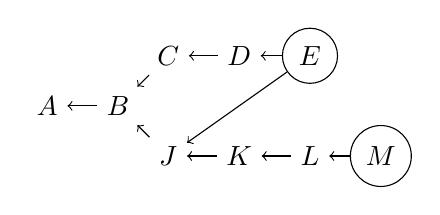
\begin{tikzpicture}[node distance=0.9cm]

% nodes
\node (a) {$A$};
\node (b) [right of=a] {$B$};
\node (c) [above right of=b] {$C$};
\node (d) [right of=c] {$D$};
\node (e) [right of=d,draw,circle] {$E$};
\node (j) [below right of=b] {$J$};
\node (k) [right of=j] {$K$};
\node (l) [right of=k] {$L$};
\node (m) [right of=l,draw,circle] {$M$};

% arrows
\draw[<-] (a) -- (b);
\draw[<-] (b) -- (c);
\draw[<-] (c) -- (d);
\draw[<-] (d) -- (e);
\draw[<-] (j) -- (e);
\draw[<-] (b) -- (j);
\draw[<-] (j) -- (k);
\draw[<-] (k) -- (l);
\draw[<-] (l) -- (m);
\end{tikzpicture}
    \caption{Messages at $p$ before reconciliation.}
    \end{subfigure}
    \begin{subfigure}{0.33\columnwidth}
    \centering
    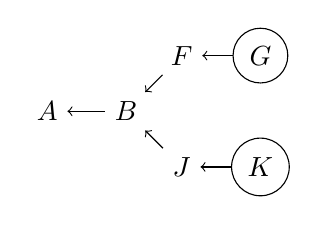
\begin{tikzpicture}

% nodes
\node (a) {$A$};
\node (b) [right of=a] {$B$};
\node (f) [above right of=b] {$F$};
\node (g) [right of=f,circle,draw] {$G$};
\node (j) [below right of=b] {$J$};
\node (k) [right of=j,circle,draw] {$K$};

% arrows
\draw[<-] (a) -- (b);
\draw[<-] (b) -- (f);
\draw[<-] (f) -- (g);
\draw[<-] (b) -- (j);
\draw[<-] (j) -- (k);
\end{tikzpicture}
    \caption{Messages at $q$ before reconciliation.}
    \end{subfigure}
    \begin{subfigure}{0.33\columnwidth}
    \centering
    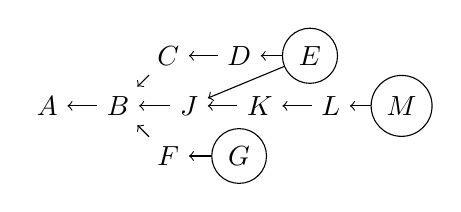
\begin{tikzpicture}[node distance=0.9cm]

% nodes
\node (a) {$A$};
\node (b) [right of=a] {$B$};
\node (c) [above right of=b] {$C$};
\node (d) [right of=c] {$D$};
\node (e) [right of=d,draw,circle] {$E$};
\node (j) [right of=b] {$J$};
\node (k) [right of=j] {$K$};
\node (l) [right of=k] {$L$};
\node (m) [right of=l,draw,circle] {$M$};
\node (f) [below right of=b] {$F$};
\node (g) [right of=f,draw,circle] {$G$};

% arrows
\draw[<-] (a) -- (b);
\draw[<-] (b) -- (c);
\draw[<-] (c) -- (d);
\draw[<-] (d) -- (e);
\draw[<-] (b) -- (j);
\draw[<-] (j) -- (e);
\draw[<-] (j) -- (k);
\draw[<-] (k) -- (l);
\draw[<-] (l) -- (m);
\draw[<-] (b) -- (f);
\draw[<-] (f) -- (g);
\end{tikzpicture}
    \caption{Messages at $p$ and $q$ after reconciliation.}
    \end{subfigure}
    \caption{Example DAGs of delivered messages. Arrows represent a message referencing the hash of its predecessor, and heads (messages with no successors) are marked with circles.}
    \label{fig:example-dags}
\end{figure}

\begin{figure}
    \vspace{0.5cm}
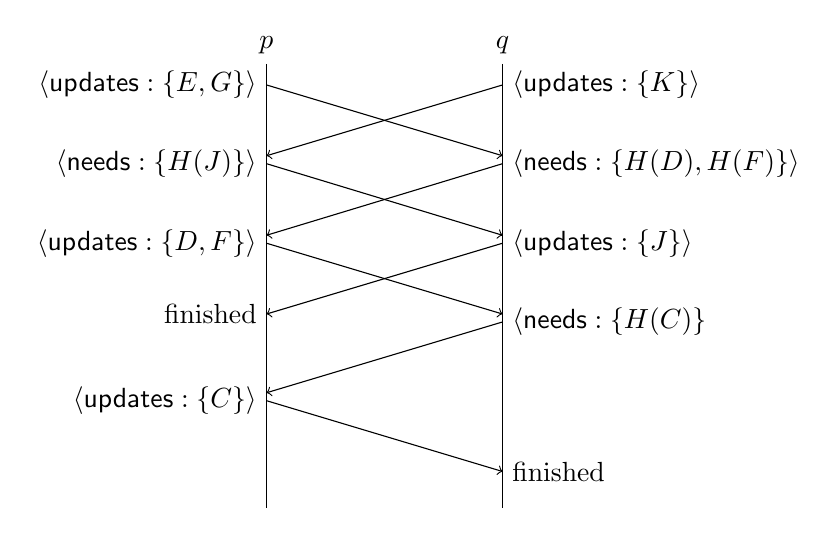
\begin{tikzpicture}
\def\width{3cm}
\def\latency{1cm}
\def\spacing{0.1cm}
\def\length{6cm}
\def\startdelay{0.5cm}

% Timelimes
\node (p1-start) at (0,0) {$p$};
\node (p2-start) at (\width,0) {$q$};
\node (p1-end) at (0,-\length) {};
\node (p2-end) at (\width,-\length) {};
\draw (p1-start) -- (p1-end);
\draw (p2-start) -- (p2-end);

% Messages
\draw[->] (0,-\startdelay) node[left] {$\langle\mathsf{updates}: \{E,G\}\rangle$} -- (\width,\spacing-\startdelay-\latency);
\draw[->] (\width,-\startdelay) node[right] {$\langle\mathsf{updates}: \{K\}\rangle$} -- (0,\spacing-\startdelay-\latency);

\draw[->] (\width, -\startdelay-\latency) node[right] {$\langle\mathsf{needs}: \{H(D), H(F)\}\rangle$} -- (0,\spacing-\startdelay-2.0\latency);
\draw[->] (0, -\startdelay-\latency) node[left] {$\langle\mathsf{needs}: \{H(J)\}\rangle$} -- (\width,\spacing-\startdelay-2.0\latency);

\draw[->] (0, -\startdelay-2.0\latency) node[left] {$\langle\mathsf{updates}: \{D, F\}\rangle$} -- (\width,\spacing-\startdelay-3.0\latency);
\draw[->] (\width, -\startdelay-2.0\latency) node[right] {$\langle\mathsf{updates}: \{J\}\rangle$} -- (0,\spacing-\startdelay-3.0\latency) node[left] {finished};

\draw[->] (\width, -\startdelay-3.0\latency) node[right] {$\langle\mathsf{needs}: \{H(C)\}$} -- (0,\spacing-\startdelay-4.0\latency);

\draw[->] (0, -\startdelay-4.0\latency) node[left] {$\langle\mathsf{updates}: \{C\}\rangle$} -- (\width,\spacing-\startdelay-5.0\latency) node[right] {finished};

\end{tikzpicture}
    \caption{Requests/responses sent in the course of running the reconciliation process in Algorithm~\ref{fig:algorithm} with the example in Figure~\ref{fig:example-dags}.}
    \label{fig:messages}
\end{figure}

We illustrate the operation of the reconciliation algorithm using the example in Figure~\ref{fig:example-dags}; the requests/responses sent in the course of the execution are shown in Figure~\ref{fig:messages}.
Initially, when a connection is established between two nodes, they send each other their heads (Algorithm~\ref{fig:algorithm}, line~\ref{line:send-heads}).
In the example of Figure~\ref{fig:example-dags}, $p$ sends $\langle\mathsf{heads}: \{H(E),H(M)\}\rangle$ to $q$, while $q$ sends $\langle\mathsf{heads}: \{H(G),H(K)\}\rangle$ to $p$.

Each node also initializes variables $\mathit{sent}$ and $\mathit{recvd}$ to contain the set of messages sent to/received from the other node within the scope of this particular connection, $\mathit{missing}$ to contain the set of hashes for which we currently lack a message, and $\mathcal{M}_\mathsf{conn}$ to contain a read-only snapshot of this node's set of messages $\mathcal{M}$ at the time the connection is established (line~\ref{line:init}).
In practice, this snapshot can be implemented using snapshot isolation~\cite{Berenson:1995}.

A node may concurrently execute several instances of this algorithm using several connections; each connection then has a separate copy of the variables $\mathit{sent}$, $\mathit{recvd}$, $\mathit{missing}$, and $\mathcal{M}_\mathsf{conn}$, while $\mathcal{M}$ is a global variable that is shared between all connections.
Each connection thread executes independently, except for the blocks marked \emph{atomically}, which are executed only by one thread at a time on a given node.
$\mathcal{M}$ should be maintained in stable storage, while the other variables may be lost in case of a crash.

On receiving the heads from the other node (line~\ref{line:recv-heads}), the recipient checks whether the recipient's $\mathcal{M}_\mathsf{conn}$ contains a matching message for each hash.
If any hashes are unknown, it replies with a $\mathsf{needs}$ request for the messages matching those hashes (lines~\ref{line:heads-missing} and \ref{line:send-missing}).
In our running example, $p$ needs $H(G)$, while $q$ needs $H(E)$ and $H(M)$.
A node responds to such a $\mathsf{needs}$ request by returning all the matching messages in a $\mathsf{msgs}$ response (lines~\ref{line:recv-needs}--\ref{line:end-needs}).

On receiving $\mathsf{msgs}$, we first discard any broadcast messages that are not correctly signed (line~\ref{line:msgs-recvd}): the function $\mathrm{check}(m, s)$ returns $\mathsf{true}$ if $s$ is a valid signature over message $m$ by a legitimate node in the system, and $\mathsf{false}$ otherwise.
For each correctly signed message we then inspect the hashes.
If any predecessor hashes do not resolve to a known message in $\mathcal{M}_\mathsf{conn}$ or $\mathit{recvd}$, the node sends another $\mathsf{needs}$ request with those hashes (lines~\ref{line:msgs-missing}--\ref{line:msgs-handle-missing}).
In successive rounds of this protocol, the nodes work their way from the heads along the paths of predecessors, until they reach the common ancestors of both nodes' heads.

Eventually, when there are no unresolved hashes, we update the global set $\mathcal{M}$ to reflect the messages we have delivered, perform a topological sort of the graph of received messages to put them in causal order, deliver them to the application in that order, and conclude the protocol run (lines~\ref{line:missing-empty}--\ref{line:finish}).
Once a node completes reconciliation (by reaching line~\ref{line:finish}), it knows that it has delivered every message that had been delivered by the other node at the time when the reconciliation started.

When a message $m$ is broadcast, it is also sent as $\langle\mathsf{msgs}: \{m\}\rangle$ on line~\ref{line:eager-send}, and the recipient treats it the same as $\mathsf{msgs}$ received during reconciliation (lines~\ref{line:recv-msgs}--\ref{line:recv-msgs-end}).
Sending messages in this way is not strictly necessary, as the periodic reconciliations will eventually deliver such messages, but broadcasting them eagerly can reduce latency.
Moreover, when a recipient delivers messages, it may also choose to eagerly relay them to other nodes it is connected to, without waiting for the next reconciliation (line~\ref{line:eager-relay}); this also reduces latency, but may result in a node redundantly receiving messages that it already has.
The literature on gossip protocols examines in detail the question of when nodes should forward messages they receive~\cite{Leitao:2009fi}, while considering trade-offs of delivery latency and bandwidth use; we leave a detailed discussion out of scope for this paper.

We prove in Appendix~\ref{sec:proof} that this algorithm implements all five properties of causal broadcast.
Even though Byzantine-faulty nodes may send arbitrarily malformed messages, a correct node will not deliver messages without a complete predecessor graph.
Any messages delivered by one correct node will eventually reach every other correct node through reconciliations.
After reconciliation, both nodes have delivered the same set of messages.

\subsection{Reducing the number of round trips}\label{sec:algorithm2}

A downside of Algorithm~\ref{fig:algorithm} is that the number of round trips can be up to the length of the longest path in the predecessor graph, making it slow when performing reconciliation over a high-latency network.
We now show how to reduce the number of round-trips using Bloom filters~\cite{Bloom:1970} and a small amount of additional state.

Note that Algorithm~\ref{fig:algorithm} does not store any information about the outcome of the last reconciliation with a particular node; if two nodes periodically reconcile their states, they need to discover each other's state from scratch on every protocol run.
As per Section~\ref{sec:system-model} we assume that communication between nodes is authenticated, and thus a node knows the identity of the other node it is communicating with.
We can therefore record the outcome of a protocol run with a particular node, and use that information in the next reconciliation with the same node.
We do this by adding the following instruction after line~\ref{line:update-m} of Algorithm~\ref{fig:algorithm}, where $q$ is the identity of the current connection's remote node:
\[ \textsc{StoreHeads}(q, \mathrm{heads}(\mathcal{M}_\mathsf{conn} \cup \mathit{recvd})) \]
which updates a key-value store in stable storage, associating the value $\mathrm{heads}(\mathcal{M}_\mathsf{conn} \cup \mathit{recvd})$ with the key $q$ (overwriting any previous value for that key if appropriate).
We use this information in Algorithm~\ref{fig:algorithm2}, which replaces the ``on connecting'' and ``on receiving heads'' functions of Algorithm~\ref{fig:algorithm}, while leaving the rest of Algorithm~\ref{fig:algorithm} unchanged.

\begin{algorithm}
    \begin{algorithmic}[1]
    \On{connecting to node $q$, and periodically}\Comment{Replaces lines \ref{line:connect-begin}--\ref{line:connect-end} of Algorithm \ref{fig:algorithm}}
        \State $\mathit{sent} := \{\};\; \mathit{recvd} := \{\};\; \mathit{missing} := \{\};\; \mathcal{M}_\mathsf{conn} := \mathcal{M}$ \Comment{connection-local variables}
        \State $\mathit{oldHeads} := \Call{LoadHeads}{q}$\label{line:load-heads}
        \State $\mathit{filter} := \textsc{MakeBloomFilter}(\Call{MessagesSince}{\mathit{oldHeads}})$\label{line:make-bloom}
        \State \textbf{send} $\langle\mathsf{heads}: \mathrm{heads}(\mathcal{M}_\mathsf{conn}),\, \mathsf{oldHeads}: \mathit{oldHeads},\, \mathsf{filter}: \mathit{filter}\rangle$ \label{line:a2-send-heads}
    \EndOn
    \State
    \On{receiving $\langle\mathsf{heads}: \mathit{hs},\, \mathsf{oldHeads}: \mathit{oldHeads},\, \mathsf{filter}: \mathit{filter}\rangle$}\Comment{Replaces lines \ref{line:recv-heads}--\ref{line:recv-heads-end} of Algorithm \ref{fig:algorithm}}\label{line:a2-recv-heads}
        \State $\mathit{bloomNegative} := \{m \in \Call{MessagesSince}{\mathit{oldHeads}} \mid \neg\Call{BloomMember}{\mathit{filter}, m}\}$\label{line:bloom-member}
        \State $\mathit{reply} := \left(\mathit{bloomNegative} \,\cup\, \bigcup_{m \in \mathit{bloomNegative}} \mathrm{succ}^*(\mathcal{M}_\mathsf{conn}, m)\right) \setminus \mathit{sent}$\label{line:bloom-succ}
        \If{$\mathit{reply} \neq \{\}$}
            \State $\mathit{sent} := \mathit{sent} \cup \mathit{reply}$
            \State \textbf{send} $\langle\mathsf{msgs}: \mathit{reply}\rangle$ \label{line:a2-heads-reply}
        \EndIf
        \State \Call{HandleMissing}{$\{h \in \mathit{hs} \mid \nexists m \in \mathcal{M}_\mathsf{conn}.\; H(m) = h\}$} \label{line:a2-heads-missing}
    \EndOn
    \State
    \Function{MessagesSince}{$\mathit{oldHeads}$}\label{line:msg-since-begin}
        \State $\mathit{known} := \{m \in \mathcal{M}_\mathsf{conn} \mid H(m) \in \mathit{oldHeads}\}$
        \State \textbf{return} $\mathcal{M}_\mathsf{conn} \setminus \left(\mathit{known} \,\cup\, \bigcup_{m \in \mathit{known}} \mathrm{pred}^*(\mathcal{M}_\mathsf{conn}, m)\right)$
    \EndFunction\label{line:msg-since-end}
    \end{algorithmic}
    \caption{Optimizing Algorithm~\ref{fig:algorithm} to reduce the number of round-trips.}\label{fig:algorithm2}
\end{algorithm}

First, when node $p$ establishes a connection with node $q$, $p$ calls $\textsc{LoadHeads}(q)$ to load the heads from the previous reconciliation with $q$ from the key-value store (Algorithm~\ref{fig:algorithm2}, line~\ref{line:load-heads}).
This function returns the empty set if this is the first reconciliation with $q$.
For example, in Figure~\ref{fig:example-dags}, the previous reconciliation heads could be $\{H(B)\}$.

In lines~\ref{line:msg-since-begin}--\ref{line:msg-since-end} of Algorithm~\ref{fig:algorithm2} we find all of the delivered messages that were added to $\mathcal{M}$ since this last reconciliation (i.e.\ all messages that are not among the last reconciliation's heads or their predecessors), and on line~\ref{line:make-bloom} we construct a Bloom filter~\cite{Bloom:1970} containing those messages.
A Bloom filter is a space-efficient data structure for testing set membership.
It is an array of $m$ bits that is initially all zero; in order to indicate that a certain element is in the set, we choose $k$ bits to set to 1 based on the hash of the element.
To test whether an element is in the set, we check whether all $k$ bits for the hash of that element are set to 1; if so, we say that the element is in the set.
This procedure may produce false positives because it is possible that all $k$ bits were set to 1 due to different elements, not due to the element being checked.
The false-positive probability is a function of the number of elements in the set, the number of bits $m$, and the number of bits $k$ that we set per element~\cite{Bloom:1970,Bose:2008,Christensen:2010}.

We assume $\textsc{MakeBloomFilter}(S)$ creates a Bloom filter from set $S$ and $\textsc{BloomMember}(F,s)$ tests if the element $s$ is a member of the Bloom filter $F$.
In the example of Figure~\ref{fig:example-dags}, $p$'s Bloom filter would contain $\{C, D, E, J, K, L, M\}$, while $q$'s filter contains $\{F, G, J, K\}$.
We send this Bloom filter to the other node, along with the heads (Algorithm~\ref{fig:algorithm2}, lines~\ref{line:make-bloom}--\ref{line:a2-send-heads}).

On receiving the heads and Bloom filter, we identify any messages that were added since the last reconciliation that are \emph{not} present in the Bloom filter's membership check (line~\ref{line:bloom-member}).
In the example, $q$ looks up $\{F, G, J, K\}$ in the Bloom filter received from $p$; \textsc{BloomMember} returns true for $J$ and $K$. \textsc{BloomMember} is likely to return false for $F$ and $G$, but may return true due to a false positive.
In this example, we assume that \textsc{BloomMember} returns false for $F$ and true for $G$ (a false positive in the case of $G$).

Any Bloom-negative messages are definitely unknown to the other node, so we send those in reply.
Moreover, we also send any successors of Bloom-negative messages (line~\ref{line:bloom-succ}): since the set $\mathcal{M}$ for a correct node cannot contain messages whose predecessors are missing, we know that these messages must also be missing from the other node.
In the example, $q$ sends $\langle\mathsf{msgs}: \{F, G\}\rangle$ to $p$, because $F$ is Bloom-negative and $G$ is a successor of $F$.

Due to Bloom filter false positives, the set of messages in the reply on line~\ref{line:a2-heads-reply} may be incomplete, but it is likely to contain most of the messages that the other node is lacking.
To fill in the remaining missing messages we revert back to Algorithm~\ref{fig:algorithm}, and perform round trips of $\mathsf{needs}$ requests and $\mathsf{msgs}$ responses until the set of messages is complete.

The size of the Bloom filter can be chosen dynamically based on the number of elements it contains.
Note that the Bloom filter reflects only messages that were added since the last reconciliation with $q$, not all messages $\mathcal{M}$.
Thus, if the reconciliations are frequent, they can employ a small Bloom filter size to minimize the cost.

This optimized algorithm also tolerates Byzantine faults.
For example, a faulty node may send a correct node an arbitrarily corrupted Bloom filter, but this only changes the set of messages in the reply from the correct node, and has no effect on $\mathcal{M}$ at the correct node.
We prove in Appendix~\ref{sec:proof} that this algorithm implements causal broadcast without making any assumption about the number of Byzantine nodes.

\subsection{Discussion}\label{sec:algorithm-discussion}

If a node crashes and restarts, or temporarily disconnects from the network, it may have missed some messages that were sent while the node was unreachable.
Our algorithm nevertheless ensures eventual delivery since a node will learn about any lost messages as it performs reconciliations with other nodes.

One further optimization could be added to our algorithms: on receiving the other node's heads, a node can check whether it has any successors of those heads.
If so, those successors can immediately be sent to the other node (Git calls this a ``fast-forward'').
If neither node's heads are known to the other (i.e.\ their histories have diverged), they fall back to the aforementioned algorithm.
We have omitted this optimization from our algorithms because we found that it did not noticeably improve the performance of Algorithm~\ref{fig:algorithm2}, and so it was not worth the additional complexity.

A potential issue with Algorithms~\ref{fig:algorithm} and~\ref{fig:algorithm2} is the unbounded growth of storage requirements, since the set $\mathcal{M}$ grows monotonically (much like most algorithms for Byzantine agreement, which produce an append-only log without considering how that log might be truncated).
If the set of nodes in the system is known, we can truncate history as follows: once every node has delivered a message $m$ (i.e.\ $m$ is \emph{stable}~\cite{Birman:1991el}), the algorithm no longer needs to refer to any of the predecessors of $m$, and so all of those predecessors can be safely removed from $\mathcal{M}$ without affecting the algorithm.
Stability can be determined by keeping track of the latest heads for each node, and propagating this information between nodes.

When one of the communicating nodes is Byzantine-faulty, the reconciliation algorithm may never terminate, e.g.\ because the faulty node may send hashes that do not resolve to any message, and so the state $\mathit{missing} = \{\}$ is never reached.
However, in a non-terminating protocol run no messages are delivered and $\mathcal{M}$ is never updated, and so the actions of the faulty node have no effect on the state of the correct node.
Reconciliations with other nodes are unaffected, since nodes may perform multiple reconciliations concurrently.
Faulty nodes could also attempt a denial-of-service attack by sending an overwhelming number of messages to correct nodes; correct nodes can defend against this by using a fair scheduling algorithm that ensures reconciliations with correct nodes continue to be processed.

In a protocol run that terminates, the only possible protocol violations from a Byzantine-faulty node are to omit heads, or to extend the set $\mathcal{M}$ with well-formed messages (i.e.\ messages containing only hashes that resolve to other messages, signed with the private key of one of the nodes in the system).
Any omitted messages will eventually be received through reconciliations with other correct nodes, and any added messages will be forwarded to other nodes; either way, the eventual delivery property of causal broadcast is preserved.

Arbitrary $\mathsf{needs}$ requests sent by a faulty node do not affect the state of the recipient.
Thus, a faulty node cannot corrupt the state of a correct node in a way that would prevent it from later reconciling with another correct node.

If one of the nodes crashes, both nodes abort the reconciliation and no messages are delivered.
The next reconciliation attempt then starts afresh.
(If desired, it would not be difficult to modify the algorithm so that an in-progress reconciliation can be restarted.)
Note that it is possible for one node to complete reconciliation and to deliver its new messages while the other node crashes just before reaching this point.
Thus, when we load the heads from the previous reconciliation on line~\ref{line:load-heads} of Algorithm~\ref{fig:algorithm2}, the local and the remote node's $\mathit{oldHeads}$ may differ.
This does not affect the correctness of the algorithm.


% TODO: evaluation should compare to libp2p/IPLD, Depot, Matrix
% (see also email from Jamie Brandon dated 28 April 2021)

\section{Experimental Evaluation}\label{sec:evaluation}

We evaluate our algorithm from Section~\ref{sec:algorithm} by comparing its performance to several existing hash graph reconciliation algorithms: two algorithms used by the Git version control system~\cite{GitHTTP,GitSkipping}, and the OldBlue~\cite{VanGundy:2012} algorithm, which is similar to our Algorithm~\ref{fig:algorithm}.
For Git, we run Git version 2.35.1 and use mitmproxy~\cite{mitmproxy} to record its communication with \texttt{github.com} using Git's ``smart'' HTTP protocol~\cite{GitHTTP}.
For OldBlue and our Algorithm~\ref{fig:algorithm2}, we implemented a prototype in JavaScript, which runs all nodes in-memory in a single process and simulates a message-passing network.
% TODO: URL of anonymised source code
To ensure a fair comparison, in the case of Git we measure only the size of HTTP request and response bodies, and we exclude overheads from HTTP headers, TLS, and TCP.

\begin{figure}
    \begin{subfigure}{0.49\columnwidth}
    \centering
    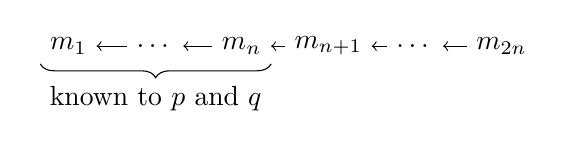
\begin{tikzpicture}[node distance=1.1cm]
\node (m1) {$m_1$};
\node (m2) [right of=m1] {\dots};
\node (m3) [right of=m2] {$m_n$};
\node (m4) [right of=m3] {$m_{n+1}$};
\node (m5) [right of=m4] {\dots};
\node (m6) [right of=m5] {$m_{2n}$};
\draw[<-] (m1) -- (m2);
\draw[<-] (m2) -- (m3);
\draw[<-] (m3) -- (m4);
\draw[<-] (m4) -- (m5);
\draw[<-] (m5) -- (m6);
\draw[decorate, decoration={brace, amplitude=5pt, mirror}] (m1.south west) -- node [below, inner sep=8pt] {known to $p$ and $q$} (m3.south east);
\end{tikzpicture}
    \caption{Hash graph at $p$ before reconciliation.}
    \end{subfigure}
    \begin{subfigure}{0.49\columnwidth}
    \centering
    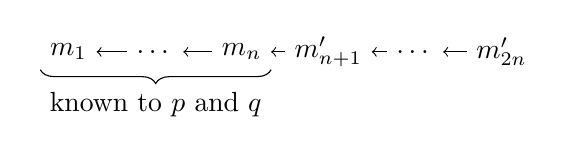
\begin{tikzpicture}[node distance=1.1cm]
\node (m1) {$m_1$};
\node (m2) [right of=m1] {\dots};
\node (m3) [right of=m2] {$m_n$};
\node (m4) [right of=m3] {$m_{n+1}'$};
\node (m5) [right of=m4] {\dots};
\node (m6) [right of=m5] {$m_{2n}'$};
\draw[<-] (m1) -- (m2);
\draw[<-] (m2) -- (m3);
\draw[<-] (m3) -- (m4);
\draw[<-] (m4) -- (m5);
\draw[<-] (m5) -- (m6);
\draw[decorate, decoration={brace, amplitude=5pt, mirror}] (m1.south west) -- node [below, inner sep=8pt] {known to $p$ and $q$} (m3.south east);
\end{tikzpicture}
    \caption{Hash graph at $q$ before reconciliation.}
    \end{subfigure}
    \caption{Reconciliation scenario used in our evaluation.}
    \label{fig:evaluation-dags}
\end{figure}

\begin{figure*}
  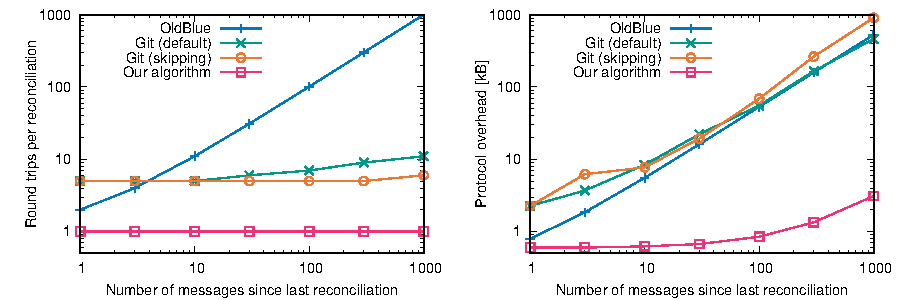
\includegraphics[width=\textwidth,keepaspectratio=true]{evaluation/comparison.pdf}
  \caption{Results from the evaluation of our prototype (lower is better). Left: number of network round trips to complete one reconciliation; right: protocol overhead, in kB, of one reconciliation.}
  \label{fig:evaluation}
\end{figure*}

In this experiment we test the scenario illustrated in Figure~\ref{fig:evaluation-dags}.
Two nodes $p$ and $q$ are assumed to have the first $n$ messages (in a linear hash chain) in common.
Then $p$ adds a further $n$ messages in a linear sequence, and $q$ independently also adds $n$ messages.
Finally, $p$ and $q$ reconcile their states, and we measure the number of round trips and the number of bytes transmitted in the course of this reconciliation.
Figure~\ref{fig:evaluation} shows the results for values of $1 \le n \le 1000$.

In this experiment we let each message be a random string of 1,000 bytes.
In Git, we simulate a message by committing a 1,000-byte random file to the repository, and we perform a reconciliation between a client node and a server node by running \texttt{git fetch} followed by \texttt{git push}.
We define the protocol overhead, shown on the right side of Figure~\ref{fig:evaluation}, to be the network traffic sent during the reconciliation, minus the total size of the messages that need to be exchanged.
For example, with $n=1000$, the total size of messages to be exchanged is 2~MB ($1000 \times 1000$ bytes in each direction); if the reconciliation sends 2.464~MB over the network then the overhead is 464~kB.

With OldBlue and our Algorithm~\ref{fig:algorithm}, which resolve one missing hash dependency at a time, the number of round trips grows linearly with the length of the longest hash chain since the last reconciliation, as expected.
The default negotiation algorithm in \texttt{git fetch} works by the client first sending its 32 most recent hashes, and then doubling the number of hashes on each subsequent request, until the client and server find a hash that they have in common.
The alternative \emph{skipping} algorithm in Git, enabled by the option \texttt{fetch.negotiationAlgorithm=skipping}, avoids sending every single hash by sending a sample of hashes from the history instead.
For small $n$, \texttt{git fetch} takes 3 round trips and \texttt{git push} another 2 round trips.
With $n=1000$ this grows to 8 round trips for \texttt{fetch} and 3 round trips for \texttt{push} in the case of the default algorithm; with the skipping algorithm the cost of the \texttt{fetch} remains at 3 round trips.

In contrast, with our Algorithm~\ref{fig:algorithm2}, a reconciliation requires a constant 1.02 round trips on average, regardless of the number of messages since the last reconciliation.
97.7\% of reconciliations with our algorithm complete in one round trip, 2.3\% require two round trips, and 0.02\% require three or more round trips.
These figures are based on using Bloom filters with 10 bits per entry and 7 hash functions, and 32-byte hashes (SHA-256).

In terms of protocol overhead, our algorithm also achieves considerably better results than the alternatives: around 1~kB, growing slowly to 3~kB with $n=1000$ (most of which is the Bloom filters).
Git's default algorithm and OldBlue have a similar overhead of 464~kB and 528~kB respectively at $n=1000$; Git's skipping algorithm has the highest overhead of 905~kB since the server unnecessarily sends the client some messages that the client already has.
With a 1,000-byte message size, this is a 45\% overhead; with a smaller message size, the percentage overhead would be greater.
For comparison, the 3~kB overhead of our algorithm is 0.15\% with 1,000-byte messages.
Thus, we can see that in terms of network performance, our Algorithm~\ref{fig:algorithm2} is close to the optimum of one round trip and zero overhead.

In our evaluation, all nodes correctly follow the protocol.
Adding Byzantine-faulty nodes may alter the shape of the predecessor graph (e.g.\ resulting in more concurrent updates than there are nodes), but we believe that this would not fundamentally alter our results.
We leave an evaluation of other metrics (e.g.\ CPU or memory use) for future work.


\section{Applications of Byzantine Causal Broadcast}\label{sec:applications}

Recent years have seen a surge in interest in decentralized peer-to-peer applications under the umbrella of ``Web3''.
Such systems aim to enable different parties to cooperate in a distributed computation without having to trust one another.
At present, these applications are typically built upon distributed ledgers (blockchains), which provide Byzantine fault tolerant total order broadcast, as explained in Section~\ref{sec:broadcast}.
However, application logic is often executed \emph{off-chain} to avoid the high costs and long delays inherent in today's blockchains.
Users have to simply trust that such off-chain computations are performed correctly, since they do not undergo the same validation process as on-chain state.

Byzantine causal broadcast offers a low-cost, lightweight alternative to distributed ledgers and total order broadcast.
For some applications, such as cryptocurrencies, causal broadcast alone is not sufficient, because it would allow the same coin to be spent in two concurrent operations, violating the rule against double-spending.
However, for many other applications, such as group communication or collaboration, and decentralized social media, causal broadcast is sufficient, and total order broadcast is unnecessarily heavyweight.
We believe that causal broadcast can be a mechanism for making off-chain computations Byzantine fault tolerant without incurring the cost of putting them on-chain.

As an example, Algorithm~\ref{fig:key-value} shows how to implement a causally consistent~\cite{Ahamad:1995}, Byzantine fault-tolerant key-value store on top of Byzantine causal broadcast.
Every write operation is broadcast as a message (line~\ref{line:set-key}); when a message is delivered (line~\ref{line:kv-deliver}), we decide how to update the delivering node's local state $S$.
If the key does not already exist in $S$, we add the key-value mapping, along with the hash of the message, to $S$ (line~\ref{line:first-update}).
If the key already exists, and the update that last set the key is a predecessor of the current message, then we overwrite the key with the new value (line~\ref{line:overwrite}).
Moreover, if the last update and the current message are concurrent (i.e.\ neither is a predecessor of the other), we also overwrite the value if the current message has a hash that is lexicographically greater than the hash of the last update.
This ensures that when two updates to the same key are concurrent, and therefore might be delivered in either order by causal broadcast, all nodes nevertheless converge to the same state $S$ regardless of the message delivery order.

\begin{algorithm}[t]
    \begin{algorithmic}[1]
    \On{request to read value for key $k$}
        \State \textbf{if} $\exists v,h.\; (k,v,h) \in S$ \textbf{then return} $v$ \textbf{else return} $\bot$ \textbf{end}
    \EndOn
    \State
    \On{request to set key $k$ to value $v$}
        \State \textbf{broadcast} $(k,v)$ by causal broadcast\label{line:set-key}
    \EndOn
    \State
    \On{delivering $m$ by causal broadcast}\label{line:kv-deliver}
        \State $((k, v), \mathit{hs}, \mathit{sig}) := m$
        \If{$\nexists v', h'.\; (k,v',h') \in S$}
            \State $S := S \,\cup\, \{(k,v,H(m))\}$\label{line:first-update}
        \ElsIf{$\exists v', h'.\; (k,v',h') \in S \,\wedge\, (h' \in \{H(m') \mid m' \in \mathrm{pred}^*(\mathcal{M}, m)\} \,\vee\, h' < H(m))$}
            \State $S := S \,\setminus\, \{(k,v',h')\} \,\cup\, \{(k,v,H(m))\}$\label{line:overwrite}
        \EndIf
    \EndOn
    \end{algorithmic}
    \caption{Creating a causally consistent key-value store using Byzantine causal broadcast}\label{fig:key-value}
\end{algorithm}

Causally consistent key-value stores are important building blocks for many applications~\cite{Lloyd:2011,Lloyd:2013,Akkoorath2016Cure,Zawirski2015SwiftCloud}, and our approach makes it possible for those applications to tolerate Byzantine faults.
Besides key-value stores, our technique can also add Byzantine tolerance to collaborative software using Conflict-free Replicated Data Types~\cite{Shapiro:2011,Sanjuan:2020}, and other distributed databases that do not need the strict ordering of total order broadcast.
Such applications include multi-user collaborative text editors~\cite{Weiss:2009ht}, note-taking tools~\cite{vanHardenberg2020PushPin}, games~\cite{vanderLinde:2017fu}, CAD applications~\cite{Lv:2018ie}, distributed filesystems~\cite{Najafzadeh:2018bw,Tao:2015gd,Kleppmann:2021}, project management tools~\cite{Kleppmann2019localfirst}, and many others.


\section{Related Work}\label{sec:relwork}

Byzantine agreement has been the subject of extensive research and has seen a recent renewal of interest due to its application in blockchains~\cite{Bano:2019}.
To tolerate $f$ faults, Byzantine agreement algorithms typically require $3f+1$ nodes~\cite{Castro:1999,Kotla:2007,Bessani:2014}, and some even require $5f+1$ nodes~\cite{Abd:2005,Martin:2006}.
This bound can be lowered, for example, to $2f+1$ if synchrony and digital signatures are assumed~\cite{Abraham:2017}. 
Most algorithms also require at least one round of communication with at least $2f+1$ nodes, incurring both significant latency and limiting availability.
Some algorithms instead take a different approach to bounding the number of failures: for example, Upright~\cite{Clement:2009} separates the number of crash failures ($u$) and Byzantine failures ($r$) and uses $2u+r+1$ nodes.
Byzantine quorum systems~\cite{Malkhi:1998} generalize from a threshold $f$ of failures to a set of possible failures.
Zeno~\cite{Singh:2009} makes progress with just $f+1$ nodes, but safety depends on less than $\frac{1}{3}$ of nodes being Byzantine-faulty.

Previous work on Secure Reliable Multicast~\cite{Malki:1996,Malkhi:2000}, Byzantine reliable broadcast~\cite{Guerraoui:2020}, Secure Causal Atomic Broadcast~\cite{Cachin:2001cj,Duan:2017}, Byzantine Lattice Agreement~\cite{DiLuna:2020}, and Byzantine fault tolerant CRDTs~\cite{Chai:2014,Shoker:2017,Zhao:2016} also assumes $3f+1$ nodes.
Byz-GentleRain~\cite{Huang:2021} and Alg Byz-RCM~\cite{Tseng:2019jb} provide causal consistency with $3f+1$ nodes.
Auvolat et al.~\cite{Auvolat:2021} provide a stronger variant of causal broadcast, which again requires $3f+1$ nodes.
All of these algorithms require Sybil countermeasures, such as central control over the participating nodes' identities; moreover, many algorithms ignore the problem of reconfiguring the system to change the set of nodes.

% Tseng et al. also claim that Byzantine causal memory requires a minimum of $3f+1$ processes

Very few algorithms target a system model with arbitrary numbers of Byzantine-faulty nodes: we are aware of OldBlue~\cite{VanGundy:2012} and Depot~\cite{Mahajan:2011}.
OldBlue is similar to our Algorithm~\ref{fig:algorithm}, and we evaluate it in Section~\ref{sec:evaluation}.
Depot uses a more complex replication algorithm involving a combination of logical clocks and hash chains to detect and recover from inconsistencies.
We attempted to include Depot in our evaluation, but we were not able to get the source code~\cite{DepotSource} running, and the available publications~\cite{Mahajan:2010,Mahajan:2011,Mahajan:2012} do not describe Depot's algorithm in sufficient detail to reproduce it.

Van der Linde et al.~\cite{vanderLinde:2020} consider causally consistent replication in the face of Byzantine faults, taking a very different approach to ours: detecting cryptographic proof of faulty behavior, and banning nodes found to be misbehaving.
This approach relies on a trusted central server and trusted hardware such as Intel SGX, whereas we do not assume any trusted components.

In SPORC~\cite{Feldman:2010wl}, BFT2F~\cite{Li:2007} and SUNDR~\cite{Mazieres:2002}, a faulty node can partition the system, preventing some nodes from ever synchronizing again, so these systems do not satisfy the \emph{eventual delivery} property of causal broadcast.
Drabkin et al.~\cite{Drabkin:2005} present an algorithm for Byzantine reliable broadcast, but it is sensitive to lost messages and does not ensure eventual delivery if nodes crash and restart.

Our reconciliation algorithm is related to the problem of computing the difference, union, or intersection between sets on remote nodes.
This problem has been studied in various domains, including peer-to-peer systems, deduplication of backups, and error-correction.
Approaches include using Bloom filters~\cite{Skjegstad:2011}, invertible Bloom filters~\cite{Goodrich:2011,Eppstein:2011} and polynomial encoding~\cite{Minsky:2003}.
However, these approaches are not designed to tolerate Byzantine faults.

The idea of referring to some data item using a cryptographic hash of its content, also known as \emph{content addressing}, is used in many systems, including Git~\cite{ProGit}, BitTorrent~\cite{Pouwelse:2005}, and IPFS~\cite{Benet:2014}.
Similarly, hash graphs are widely used: in Git~\cite{GitHTTP}, Matrix~\cite{Jacob:2021b}, Merkle trees~\cite{Merkle:1987}, blockchains~\cite{Bano:2019}, and peer-to-peer storage systems such as IPLD~\cite{IPLD}.
Other authors~\cite{Baird:2016tq,Kang:2003} also discuss replicated hash graphs but do not present efficient reconciliation algorithms for bringing nodes up-to-date.
Merkle-CRDTs~\cite{Sanjuan:2020} use a graph reconciliation algorithm equivalent to our unoptimized Algorithm~\ref{fig:algorithm}.

Non-Byzantine causal broadcast was introduced by the ISIS system~\cite{Birman:1991el}.
There are many non-Byzantine systems that provide causal consistency, including COPS~\cite{Lloyd:2011}, Eiger~\cite{Lloyd:2013}, Cure~\cite{Akkoorath2016Cure}, and SwiftCloud~\cite{Zawirski2015SwiftCloud}.
These systems eschew linearizability and total ordering for the sake of availability or performance; our work shows that in a Byzantine context, system designers can make a similar trade-off, forsaking total order to gain the ability to tolerate an unbounded number of Byzantine nodes.

% This one is confusing
% https://arxiv.org/abs/2112.11337

% Decentralized Collaborative Version Control
% https://dl.acm.org/doi/abs/10.1145/3493426.3493824

% BAR Gossip uses a model of "rational" nodes that are assumed to maximise a given loss function
% Harry C. Li, Allen Clement, et al. BAR Gossip. OSDI 2006 https://static.usenix.org/event/osdi06/tech/full_papers/li/li.pdf

% Secure Scuttlebutt~\cite{Kermarrec:2020} also uses hash chains, but it relies on vector clocks for replication, so it suffers from the problem illustrated in Figure~\ref{fig:vectorclocks}.

% Some more suggestions for related work (including Minisketch) in this thread: https://news.ycombinator.com/item?id=25278128
% https://github.com/sipa/minisketch
% Minisketch is proposed for gossip in Bitcoin: https://arxiv.org/abs/1905.10518
% See email from Greg Maxwell on 10 Nov 2021

% Consider cuckoo filters or quotient filters?
% https://en.wikipedia.org/wiki/Quotient_filter

% Comparison to Julien Quintard work on byzantine file systems https://www.repository.cam.ac.uk/bitstream/handle/1810/243442/thesis.pdf?sequence=1&isAllowed=y
% https://infinit.sh

% Comparison to irmin
% https://mirage.github.io/irmin/irmin/Irmin/index.html#syncing-with-a-remote
% https://github.com/mirage/irmin/blob/master/src/irmin/sync_ext.ml#L86-L123
% Send paper to Irmin authors?


\section{Conclusions}\label{sec:conc}

Many peer-to-peer systems tolerate only a bounded number of Byzantine-faulty nodes, and therefore need to employ expensive countermeasures against Sybil attacks, such as proof-of-work, or centrally controlled permissions for joining the system.
In this work, we have demonstrated that some applications can tolerate arbitrary numbers of Byzantine faults by utilizing Byzantine causal broadcast, and are therefore immune to Sybil attacks.
We highlighted some of those applications in Section~\ref{sec:applications}.

We believe that our approach will make it viable to use Byzantine fault tolerance in applications where the cost of using on-chain operations in a totally ordered distributed ledger is currently prohibitive.
For systems that currently require all nodes to be trusted, and hence can only be deployed in trusted datacenter networks, adding Byzantine fault tolerance opens up new opportunities for deployment in untrusted peer-to-peer settings.
Our algorithm is fairly simple, and it provides considerably better performance than the alternatives we evaluated in Section~\ref{sec:evaluation}.

We hope that this work will inspire further research to ensure the correctness of decentralized systems in the presence of arbitrary numbers of Byzantine faults.
Some open questions include:
\begin{itemize}
    \item How can we best ensure that correct nodes form a connected component, as assumed in Section~\ref{sec:system-model}?
    Connecting each node to every other is the simplest solution, but it can be expensive if the number of nodes is large.
    \item Can we take existing non-Byzantine distributed applications and retrofit Byzantine fault tolerance using the protocols described in this paper?
\end{itemize}

\begin{acks}
Thank you to Alastair Beresford, Jon Crowcroft, Srinivasan Keshav, Smita Vijaya Kumar and Gavin Stark for feedback on a draft of this paper.
Martin Kleppmann is supported by a Leverhulme Trust Early Career Fellowship, the Isaac Newton Trust, and Nokia Bell Labs.
This work was funded in part by EP/T022493/1.
\end{acks}

\bibliographystyle{ACM-Reference-Format}
\bibliography{references}
\appendix

\section{Proof of Correctness}\label{sec:proof}

In this appendix we show that Algorithms~\ref{fig:algorithm} and \ref{fig:algorithm2} implement causal broadcast, as defined in Section~\ref{sec:broadcast}, in the Byzantine system model of Section~\ref{sec:system-model}.
Where a lemma does not specify which of the two algorithms it applies to, it holds for both.

% self-delivery, eventual delivery, authenticity, non-duplication, causal order
\begin{lemma}\label{lemma:easy-properties}
Algorithms~\ref{fig:algorithm} and \ref{fig:algorithm2} satisfy the \emph{self-delivery}, \emph{authenticity}, \emph{non-duplication}, and \emph{causal order} properties of causal broadcast, as defined in Section~\ref{sec:broadcast}.
\end{lemma}
\begin{proof}
The \emph{self-delivery} property holds trivially, because each time a correct node broadcasts a message, it immediately delivers that message to itself (Algorithm~\ref{fig:algorithm}, line~\ref{line:deliver-local}).

The \emph{authenticity} property holds because when a broadcast message is delivered, it was either sent by the local node (Algorithm~\ref{fig:algorithm}, line~\ref{line:deliver-local}), in which case it is trivially authentic, or it was received from another node (Algorithm~\ref{fig:algorithm}, line~\ref{line:deliver}).
In the latter case, messages are in the set $\mathcal{M}$ only if they were broadcast, and we discard any messages that do not have a valid signature from its sender (Algorithm~\ref{fig:algorithm}, line~\ref{line:msgs-recvd}).
Our system model assumes that signatures are unforgeable, so a correct node delivers a message only if it was broadcast by the node that signed it.

The \emph{non-duplication} property holds because every message is unique (due to the inclusion of the hashes of its predecessors), and messages delivered during reconciliation are limited to those not already in $\mathcal{M}$ (Algorithm~\ref{fig:algorithm}, line~\ref{line:deliver}).
Since $\mathcal{M}$ is immediately updated to include all delivered messages, and this takes place in an \emph{atomic} block (preventing two threads from concurrently trying to deliver the same message), this algorithm ensures that no correct node delivers the same message more than once.

The \emph{causal order} property holds because when a correct node broadcasts a message, the predecessor hashes are computed such that every message previously broadcast or delivered by this node becomes a (direct or indirect) predecessor of the new message (Algorithm~\ref{fig:algorithm}, line \ref{line:broadcast-heads}).
Any correct node delivers messages in topologically sorted order, i.e.\ any predecessors of $m$ are delivered before $m$ (Algorithm~\ref{fig:algorithm}, line \ref{line:deliver}).
The reconciliation algorithm delivers messages only once all hashes have been resolved (once all direct and indirect predecessor messages have been received), so we know that there are no missing predecessors.
Thus, whenever a correct node broadcasts or delivers $m_1$ before broadcasting $m_2$, all correct nodes deliver $m_1$ before delivering $m_2$.
\end{proof}

This leaves the \emph{eventual delivery} property, which is the focus of the remainder of this appendix.
We consider two correct nodes $p$ and $q$, with initial sets of messages $\mathcal{M}_p$ and $\mathcal{M}_q$ respectively at the start of the execution.
Assume that in this run of the algorithm, $p$ and $q$ both complete the reconciliation by reaching line~\ref{line:finish} of Algorithm~\ref{fig:algorithm}.
Let $\mathit{recvd}_p$ be the contents of the variable $\mathit{recvd}$ at node $p$ when the reconciliation is complete, and likewise $\mathit{recvd}_q$ at node $q$.
Further, let $\mathcal{M}'_p = \mathcal{M}_p \cup \mathit{recvd}_p$ and $\mathcal{M}'_q = \mathcal{M}_q \cup \mathit{recvd}_q$ be the final set of messages at both nodes.

\begin{lemma}\label{lemma:no-p-missing}
The set of messages $\mathcal{M}$ of a correct node $p$ grows monotonically.
\end{lemma}
\begin{proof}
The node $p$ only modifies $\mathcal{M}$ by generating new operations, which are added to $\mathcal{M}$ (Algorithm~\ref{fig:algorithm}, line~\ref{line:update-m-local}), or by unioning it with the set $\mathit{recvd}$ (Algorithm~\ref{fig:algorithm}, line~\ref{line:update-m}).
Thus, elements are only added to the set $\mathcal{M}$, and therefore $\mathcal{M}$ grows monotonically.
\end{proof}

\begin{lemma}\label{lemma:no-dangling}
Let $m = (v, \mathit{hs}, \mathit{sig})$ such that $m \in \mathcal{M}_p$.
Then its predecessors are also in $\mathcal{M}_p$, i.e.\ $\forall h \in \mathit{hs}.\; \exists m' \in \mathcal{M}_p.\; H(m') = h$.
\end{lemma}
\begin{proof}
There are two ways $m$ can become a member of $\mathcal{M}_p$ for a correct node $p$:
\begin{description}
    \item[Case] $m$ is broadcast by node $p$:\\
    In this case, since $p$ is assumed to be correct, the hashes $\mathit{hs}$ are computed as $\mathit{hs} = \{H(m') \mid m' \in \mathcal{M} \wedge \mathrm{succ}^1(\mathcal{M}, m') = \{\}\,\}$ for some earlier state $\mathcal{M}$ (Algorithm~\ref{fig:algorithm}, line~\ref{line:broadcast-heads}).
    As $\mathcal{M}$ grows monotonically (Lemma~\ref{lemma:no-p-missing}), $\mathcal{M} \subseteq \mathcal{M}_p$, and thus we can deduce that $\forall h \in \mathit{hs}.\; \exists m' \in \mathcal{M}_p.\; H(m') = h$.
    \item[Case] $m$ is received from another node (which may be faulty):\\
    During the run of the protocol at which $p$ received $m$, we have $m \in \mathit{recvd}$ and $\mathit{missing} = \{\}$ at line~\ref{line:update-m} of Algorithm~\ref{fig:algorithm}.
    Let $\mathcal{M}$ be the set of messages at $p$ immediately before that execution of line~\ref{line:update-m}.
    From $\mathit{missing} = \{\}$ and line~\ref{line:msgs-missing} of Algorithm~\ref{fig:algorithm} we have $\forall h \in \mathit{hs}.\; \exists m' \in (\mathcal{M} \cup \mathit{recvd}).\; H(m') = h$.
    Since $\mathcal{M}$ grows monotonically (Lemma~\ref{lemma:no-p-missing}) and $\mathit{recvd} \subseteq \mathcal{M}_p$ (Algorithm~\ref{fig:algorithm}, line~\ref{line:update-m}), $\forall h \in \mathit{hs}.\; \exists m' \in \mathcal{M}_p.\; H(m') = h$.
\end{description}
\end{proof}

\begin{lemma}\label{lemma:no-collision}
Let $m = (v, \mathit{hs}, \mathit{sig})$ such that $m \in \mathcal{M}_p$ and $m \in \mathcal{M}_q$.
Then the hashes $\mathit{hs}$ resolve to the same messages at $p$ and $q$, that is, $\{m' \in \mathcal{M}_p \mid H(m') \in \mathit{hs}\} = \{m' \in \mathcal{M}_q \mid H(m') \in \mathit{hs}\}$.
\end{lemma}
\begin{proof}
We use proof by contradiction.
Assume there exists $h \in \mathit{hs}$ such that $\{m' \in \mathcal{M}_p \mid H(m') = h\} \neq \{m' \in \mathcal{M}_q \mid H(m') = h\}$.
By Lemma~\ref{lemma:no-dangling} we have $\{m' \in \mathcal{M}_p \mid H(m') = h\} \neq \{\}$ and similarly, $\{m' \in \mathcal{M}_q \mid H(m') = h\} \neq \{\}$.
Hence, there exist $m' \in \mathcal{M}_p$ and $m'' \in \mathcal{M}_q$ such that $m' \neq m''$ and $H(m') = H(m'') = h$.
However, this contradicts our assumption in Section~\ref{sec:algorithm} that the hash function $H(\cdot)$ is collision-resistant.
\end{proof}

\begin{lemma}\label{lemma:no-q-missing}
$\mathcal{M}_q \subseteq \mathcal{M}'_p$ when executing Algorithm~\ref{fig:algorithm}.
\end{lemma}
\begin{proof}
We use proof by contradiction.
Assume to the contrary that $\exists m \in \mathcal{M}_q.\; m \notin  \mathcal{M}'_p$.
Since $\mathit{recvd} \subseteq \mathcal{M}'_p$ and elements are only added to $\mathit{recvd}$ (Algorithm~\ref{fig:algorithm}, line~\ref{line:msgs-recvd}) then $m \notin  \mathcal{M}'_p$ implies that $m \notin \mathit{recvd}$ on node $p$.
We now consider two cases depending on the value returned by $\mathrm{succ}^1(\mathcal{M}_q, m)$:
\begin{description}
    \item[Case] $\mathrm{succ}^1(\mathcal{M}_q, m) = \{\}$:\\
    In this case, $H(m) \in \mathrm{heads}(\mathcal{M}_q)$, and so the first $\mathsf{heads}$ request from $q$ to $p$ will contain $H(m)$ (Algorithm~\ref{fig:algorithm}, line~\ref{line:send-heads}).
    Since $m \notin \mathcal{M}_p$, node $p$ will send a $\mathsf{needs}$ request to $q$ containing $H(m)$ (Algorithm~\ref{fig:algorithm}, line~\ref{line:heads-missing}).
    Upon receiving the $\mathsf{needs}$ message containing $H(m)$, node $q$ will reply with an $\mathsf{msgs}$ response containing $m$ (Algorithm~\ref{fig:algorithm}, line~\ref{line:send-msgs}).
    Node $p$ will receive the $\mathsf{msgs}$ response with $m$ from node $q$ and will add $m$ to $\mathit{recvd}$ (Algorithm~\ref{fig:algorithm}, line~\ref{line:msgs-recvd}).
    This contradicts our previous finding that $m \notin \mathit{recvd}$.
    
    \item[Case] $\mathrm{succ}^1(\mathcal{M}_q, m) \ne \{\}$:\\
    In this case, $H(m) \notin \mathrm{heads}(\mathcal{M}_q)$.
    Since $\mathcal{M}_q$ is a DAG, there must exist a message $m'$ such that $H(m') \in \mathrm{heads}(\mathcal{M}_q)$ and $m' \in \mathrm{succ}^*(\mathcal{M}_q, m)$.
    As in the previous case, $H(m') \in \mathrm{heads}(\mathcal{M}_q)$ implies that $m' \in \mathit{recvd}$.
    Note that none of the messages in $\mathrm{succ}^*(\mathcal{M}_q, m)$ are in $\mathcal{M}_p$ as $m \notin \mathcal{M}'_p$ implies that  $m \notin \mathcal{M}_p$ (Lemma~\ref{lemma:no-p-missing}).
    If $m' \in \mathrm{succ}^1(\mathcal{M}_q, m)$ then it must the case that $m \in \mathit{recvd}$ by the time that $\mathit{missing} = \emptyset$, otherwise $m \in \mathit{missing}$ (Algorithm~\ref{fig:algorithm}, line~\ref{line:msgs-missing}).
    By induction over the path of successors from $m'$ to $m$, we observe that $m \in \mathit{recvd}$.
    At each step of the induction, the nodes move to the predecessors of the previous step; due to Lemma~\ref{lemma:no-collision}, $p$ and $q$ agree about the identity of these predecessors.
    This contradicts our previous finding that $m \notin \mathit{recvd}$.
\end{description}
\end{proof}

\begin{lemma}\label{lemma:no-q-missing2}
$\mathcal{M}_q \subseteq \mathcal{M}'_p$ when executing Algorithm~\ref{fig:algorithm2}.
\end{lemma}
\begin{proof}
We use proof by contradiction.
Assume $m \in \mathcal{M}_q$ such that $m \notin \mathcal{M}_p'$ and $m \notin \mathit{recvd}$ like in Lemma~\ref{lemma:no-q-missing}.
Let $\mathit{filter}$ be the Bloom filter in the initial message from $p$ to $q$ in the current protocol run (Algorithm~\ref{fig:algorithm2}, line~\ref{line:make-bloom}).
Even though $m \notin \mathcal{M}_p$ (by Lemma~\ref{lemma:no-p-missing}), $\textsc{BloomMember}(\mathit{filter}, m)$ may return a false positive.
Moreover, if it returns true, $m$ may or may not be a successor of a $\mathit{bloomNegative}$ item as computed in Algorithm~\ref{fig:algorithm2}, lines~\ref{line:bloom-member}--\ref{line:bloom-succ}.
As a result it is possible that either $m \in \mathit{reply}$ or $m \notin \mathit{reply}$ after $q$ has executed line~\ref{line:bloom-succ} of Algorithm~\ref{fig:algorithm2}.

If $m \in \mathit{reply}$ then $p$ will receive an $\mathsf{msgs}$ response containing $m$ from $q$, which will be added to $\mathit{recvd}$, contradicting our assumption that $m \notin \mathit{recvd}$.
If $m \notin \mathit{reply}$ we continue to line~\ref{line:a2-heads-missing} of Algorithm~\ref{fig:algorithm2}, from which point onward the algorithm is the same as Algorithm~\ref{fig:algorithm}.
Thus, we have $\mathcal{M}_q \subseteq \mathcal{M}'_p$ by Lemma~\ref{lemma:no-q-missing}.
\end{proof}

\begin{lemma}\label{lemma:no-extras}
$\mathcal{M}'_p \subseteq \mathcal{M}_p \cup \mathcal{M}_q$.
\end{lemma}
\begin{proof}
We use proof by contradiction.
Assume to the contrary that $\exists m \in \mathcal{M}'_p.\; m \notin \mathcal{M}_p  \land  m \notin \mathcal{M}_q$.
Since $\exists m \in \mathcal{M}'_p$, node $p$ must have received a message containing $m$ from node $q$ before it completed reconciliation (Algorithm~\ref{fig:algorithm}, lines \ref{line:recv-msgs}--\ref{line:msgs-handle-missing} and \ref{line:update-m}).
Node $q$ will only send a message containing $m$ if $m \in \mathcal{M}_q$ or $m \in \mathcal{M}'_q$, depending on whether node $q$ has completed the reconciliation algorithm.
Since $m \notin \mathcal{M}_q$ then node $q$ must have received a message containing $m$ from node $p$.
Since $m \notin \mathcal{M}_p$ then node $p$ will not send this message and therefore $m$ does not exist.
\end{proof}

\begin{lemma}\label{lemma:reconcile-equal}
When two correct nodes $p$ and $q$, with initial sets of messages $\mathcal{M}_p$ and $\mathcal{M}_q$, have completed reconciliation (i.e.\ both have reached line~\ref{line:finish} of Algorithm~\ref{fig:algorithm}), then their final sets of messages $\mathcal{M}'_p$ and $\mathcal{M}'_q$  are both equal to $\mathcal{M}_p \cup \mathcal{M}_q$.
\end{lemma}
\begin{proof}
We have $\mathcal{M}_p \subseteq \mathcal{M}'_p$ by Lemma \ref{lemma:no-p-missing}, $\mathcal{M}_q \subseteq \mathcal{M}'_p$ by Lemmata \ref{lemma:no-q-missing} and \ref{lemma:no-q-missing2}, and $\mathcal{M}'_p \subseteq \mathcal{M}_p \cup \mathcal{M}_q$ by Lemma \ref{lemma:no-extras}.
From these facts we have shown that $\mathcal{M}'_p = \mathcal{M}_q \cup \mathcal{M}_q$.
Similarly, by swapping $p$ and $q$ we can show that $\mathcal{M}'_q = \mathcal{M}_q \cup \mathcal{M}_q$.
\end{proof}

\begin{lemma}\label{lemma:termination}
If two correct nodes attempt reconciliation an infinite number of times, then there is an infinite number of protocol runs in which the algorithm terminates (i.e.\ both nodes reach line~\ref{line:finish} of Algorithm~\ref{fig:algorithm}), assuming the system model of Section~\ref{sec:system-model}.
\end{lemma}
\begin{proof}
Our system model assumes network communication is reliable, but it allows correct nodes to crash and recover.
If a crash occurs during a reconciliation, that reconciliation may be aborted.
However, if we perform reconciliation an infinite number of times, then only a subset of reconciliations will be affected by crashes, and an infinite number of reconciliations will be free from crashes.

The graph of messages $\mathcal{M}_p$ at any correct node $p$ is finite and contains no cycles.
Therefore, every vertex $m' \in \mathcal{M}_p$ can be reached in a finite number of steps by starting a graph traversal at $\mathrm{heads}(\mathcal{M}_p)$ and, in each step, moving from each vertex to its predecessors.
Moreover, by Lemma~\ref{lemma:no-dangling}, $\mathcal{M}_p$ at any correct node $p$ contains only hashes that are the hash of another message in $\mathcal{M}_p$.
Hence, in a connection in which neither node crashes, the algorithm will always reach the state $\mathit{missing} = \{\}$ and terminate (i.e.\ reach line~\ref{line:finish} of Algorithm~\ref{fig:algorithm}) in a finite number of round-trips of $\mathsf{needs}$ requests and $\mathsf{msgs}$ responses.

Since there are an infinite number of connection attempts that are free from crashes, and the algorithm always terminates for these connections, we can conclude that there are an infinite number of protocol runs in which the algorithm terminates.
\end{proof}

\begin{theorem}
Algorithms~\ref{fig:algorithm} and~\ref{fig:algorithm2} implement causal broadcast, as defined in Section~\ref{sec:broadcast}, in the Byzantine system model of Section~\ref{sec:system-model}.
\end{theorem}
\begin{proof}
Lemma~\ref{lemma:easy-properties} proves the properties apart from \emph{eventual delivery}.
To prove eventual delivery, for any two correct nodes $p$ and $q$, we must show that a message delivered by $p$ will also be delivered by $q$.
We assume in Section~\ref{sec:system-model} that the correct nodes form a connected component in the graph of nodes and network links.
Thus, either there is a direct network link between $p$ and $q$, or there is a path of network links on which all of the intermediate links are also correct.

Assume that any two adjacent nodes on this path periodically attempt a reconciliation without a bound on the number of reconciliations.
Thus, in an execution of infinite duration, there will be an infinite number of reconciliations between any two adjacent nodes.
By Lemma~\ref{lemma:termination}, an infinite number of these reconciliations will complete.
By Lemma~\ref{lemma:reconcile-equal}, at the instant in which one of these reconciliations completes, the set of messages delivered by one node equals the set of messages delivered by the other node, with the exception of any messages delivered by concurrent reconciliations.

Any messages delivered by one node while the reconciliation with the other node was in progress will be sent in the next reconciliation, which always exists, since we are assuming an infinite number of reconciliations.
After a reconciliation where one node completes while the other does not (e.g.\ due to a crash just before completing), the sets of messages delivered by the two nodes may be different, but again the missing messages will be sent in the next reconciliation.

Let $m$ be a message that has been delivered by $p$ at some point in time.
We have $m \in \mathcal{M}_p$ from that time onward, since $\mathcal{M}_p$ is exactly the set of delivered messages, and it grows monotonically (Lemma~\ref{lemma:no-p-missing}).
Thus, $m$ will eventually be delivered by any correct node to which $p$ has a direct network link.
These nodes will eventually relay $m$ to their direct neighbors, and so on, until $m$ is delivered to $q$ through successive reconciliations along the path from $p$ to $q$.
Therefore, $m$ is eventually delivered by $q$.
\end{proof}

\end{document}
